
\section{Overview:}

This chapter describes the design methodology, architectural approach, and key technical decisions made during the development of the Breadit hybrid social networking platform. The methodology centers on a systems engineering approach: each architectural decision is evaluated against concrete alternatives based on the platform's defined requirements - real-time content delivery, hybrid feed ranking, threaded discussion management, and community moderation.

The implementation follows a TypeScript-first monorepo strategy using Turborepo, comprising two independently deployable applications: a NestJS/Fastify backend and a Next.js 15 frontend. All major technical choices - architecture pattern, pagination strategy, real-time protocol, and rendering model - are justified by explicit trade-off analysis documented in the sections below.

\section{Development Process:}

\subsection{Architecture Design:}

\begin{longtable}{|p{0.3\linewidth}|p{0.3\linewidth}|p{0.3\linewidth}|}
\caption{Table 16} \label{tab:16} \\
\hline
\textbf{Criterion} & \textbf{Modular Monolith (Chosen)} & \textbf{Microservices} \\
\hline
\endfirsthead
\multicolumn{3}{l}{\textit{(Continued from previous page)}} \\
\hline
\textbf{Criterion} & \textbf{Modular Monolith (Chosen)} & \textbf{Microservices} \\
\hline
\endhead
\hline \multicolumn{3}{r}{\textit{Continued on next page}} \\
\endfoot
\hline
\endlastfoot
Deployment complexity & Single deployable unit per application & Each service requires independent orchestration (Docker Compose, Kubernetes) \\
\hline
Inter-module communication & Direct in-process function calls via NestJS DI & Network calls (REST/gRPC), introducing latency and failure points \\
\hline
Data access & Single shared Prisma client with transactional integrity & Each service manages its own database, requiring distributed transaction patterns (SAGA) \\
\hline
Development overhead & Low - suitable for a single-developer pre-thesis project & High - requires service discovery, API gateways, and distributed logging \\
\hline
Module boundary enforcement & NestJS module encapsulation prevents cross-domain coupling & Enforced by network isolation \\
\hline
Scalability & Horizontal scaling via load balancer; Redis adapter enables stateless instances & Fine-grained per-service scaling \\
\hline
\end{longtable}

\begin{figure}[H]
  \centering
  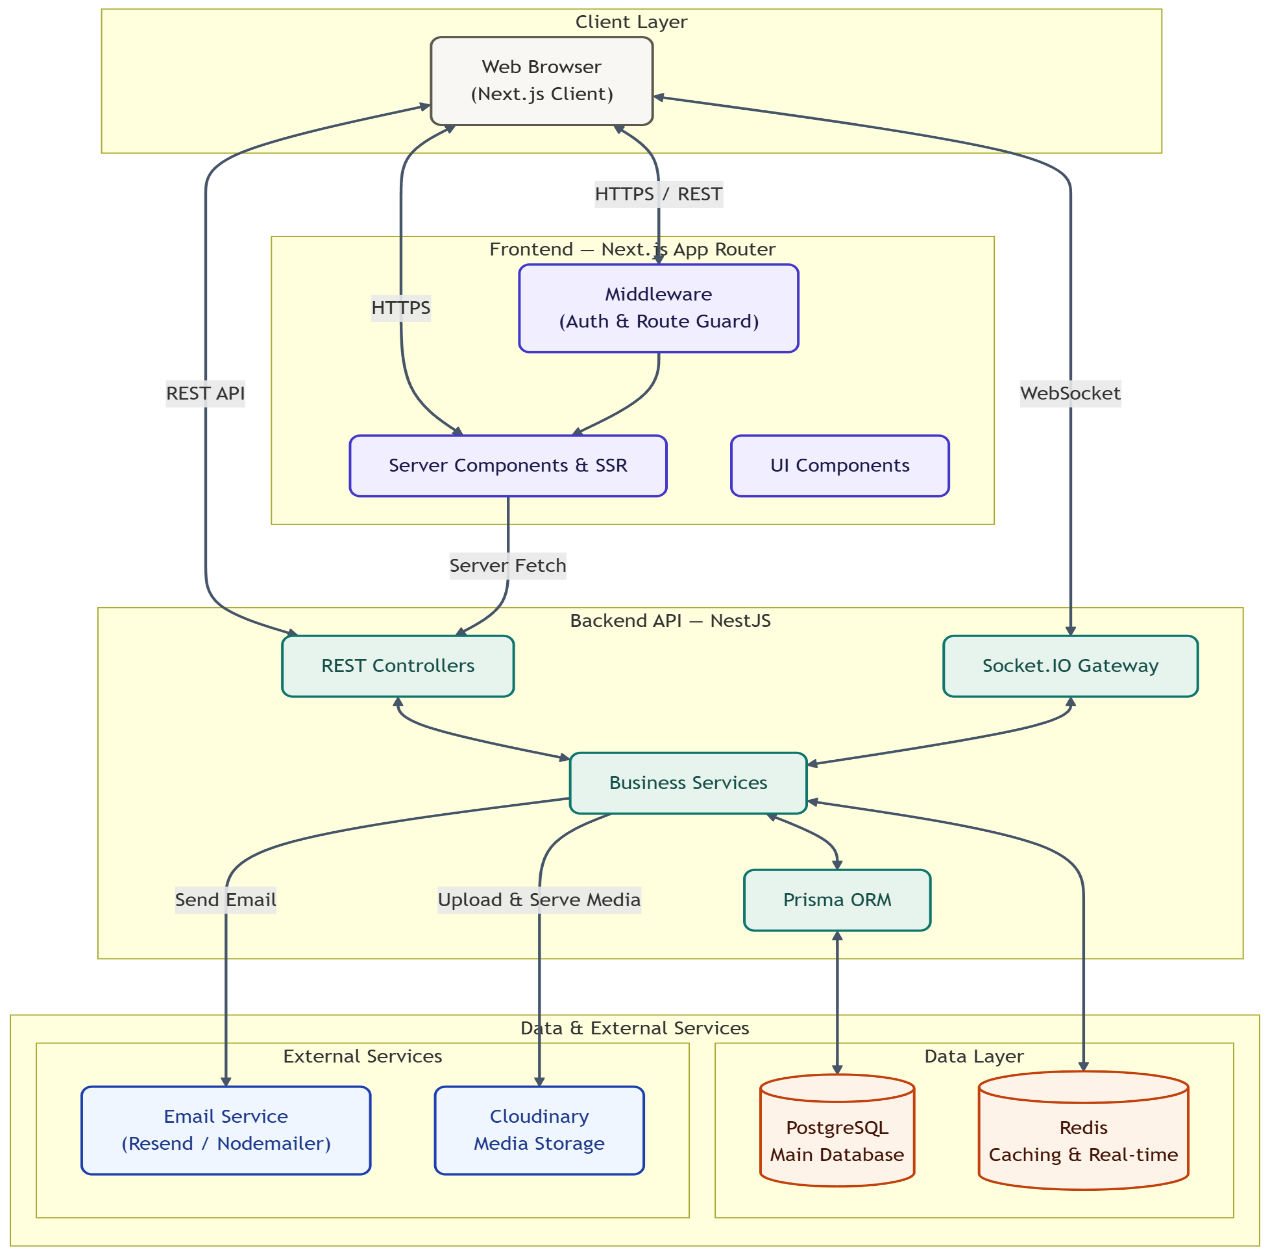
\includegraphics[width=0.92\linewidth,height=0.82\textheight,keepaspectratio]{images/image4.png}
  \caption{High-level architecture diagram}
  \label{fig:1}
\end{figure}

\textbf{Justification}: The Modular Monolithic pattern provides equivalent module isolation to Microservices while eliminating the operational overhead of distributed service orchestration. The NestJS module system enforces strict dependency injection boundaries, preventing domain coupling without requiring network-level separation. Horizontal scalability is still achievable via load-balanced deployments with the Redis-backed Socket.IO adapter, which maintains stateless WebSocket sessions.

\subsubsection{Summary Use Case:}
\begin{enumerate}
  \item Authentication: Guests and users can create accounts, securely log in, verify their email addresses, and reset their passwords.
  \item Content Discovery: Visitors and users can browse chronological feeds and search for specific users, hashtags, or communities.
  \item Post Management: Users can create new posts with rich media attachments, embed hashtags, and edit or delete their own content.
  \item Post Interaction: Users can actively engage with the platform by liking, commenting, replying to threads, reposting, and saving posts.
  \item Relationship Management: Users can follow or unfollow other profiles to curate their personal feed, and block or unblock users for privacy.
  \item Profile Management: Users can update their personal public profiles, including display name, bio, and avatar, and view their activity history.
  \item Direct Messaging: Users can communicate privately with other members through real-time direct messages.
  \item Real-time Notifications: Users receive instant system alerts for social interactions such as new followers, likes, comments, and messages.
  \item Community Management: Users can create specialized communities, join or leave existing groups, and manage community rules and members.
  \item Administrative Moderation: System administrators hold elevated privileges to manage user accounts, apply global bans, and resolve content reports.
\end{enumerate}
\begin{figure}[H]
  \centering
  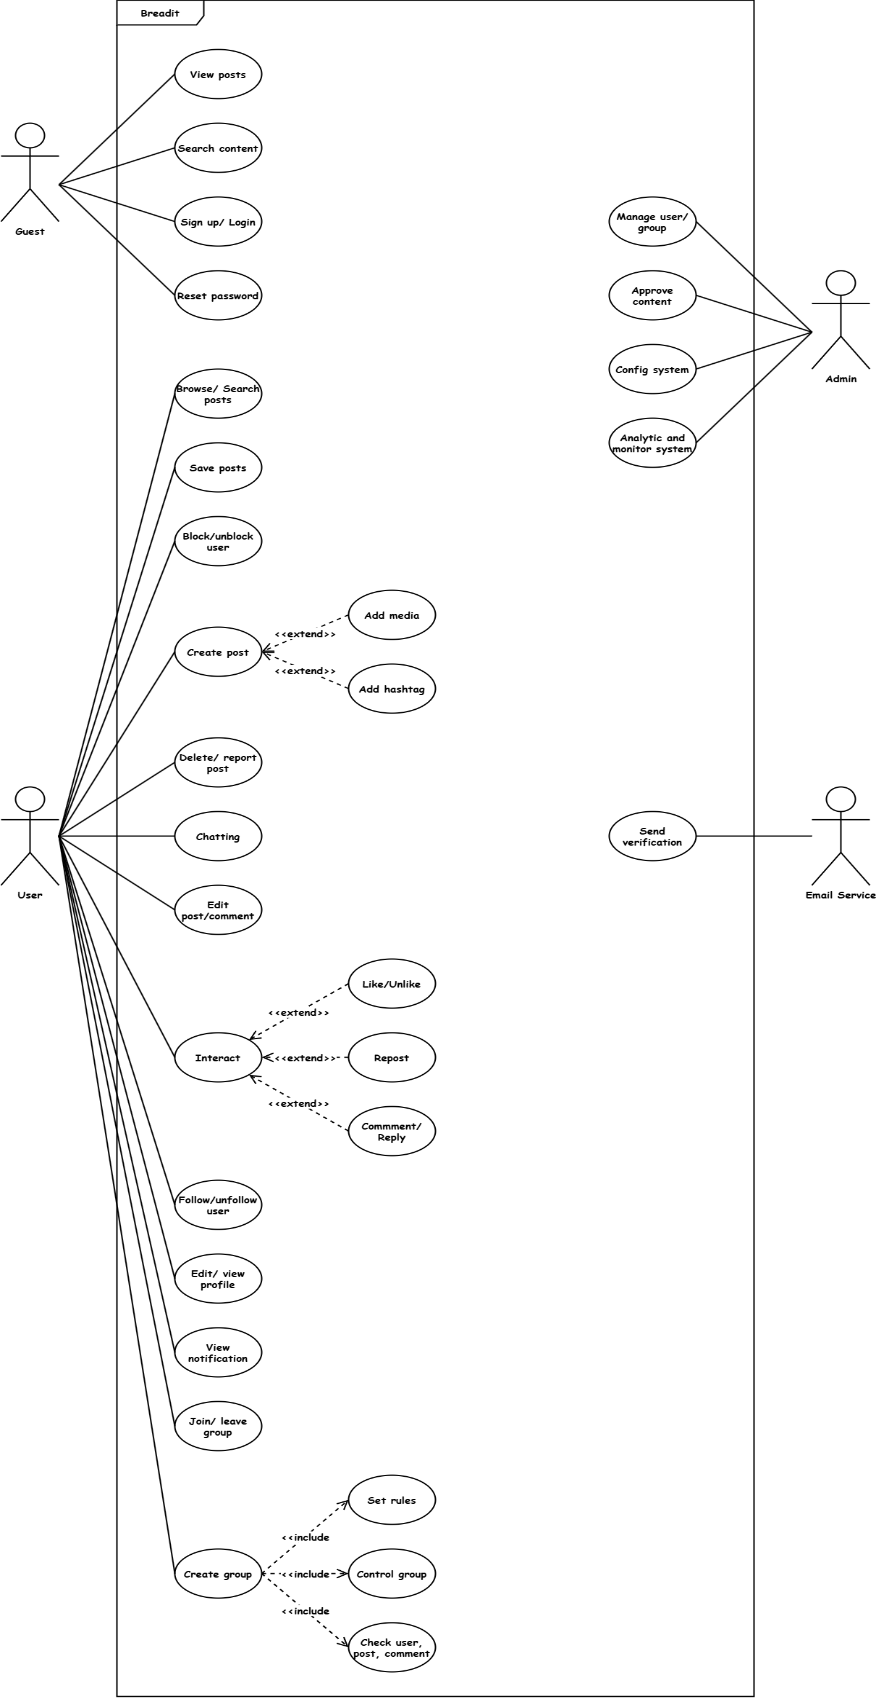
\includegraphics[width=0.92\linewidth,height=0.82\textheight,keepaspectratio]{images/image5.png}
  \caption{Summary Goal Use Case}
  \label{fig:2}
\end{figure}

Actors:
\begin{enumerate}
  \item \textbf{Guest / Unregistered User:}~Can browse public feeds, view user profiles.
  \item \textbf{User / Registered User:}~Can publish micro-blogs, actively interact with content, manage personal connections, send direct messages, and participate in communities.
  \item \textbf{System Admin:}~Manages the platform's integrity by reviewing user-reported content, resolving community disputes, and applying global bans accounts.
\end{enumerate}

\subsubsection{Use Cases:}
\begin{enumerate}
  \item Sign Up/ Login\textbf{:}~Visitors can register a new account to become users.
  \item Verify Email: Users must submit a secure code to verify emails.
  \item Password Recovery: Users can securely reset forgotten passwords via email links.
  \item Manage Profile: Users can update their public bio, avatar, and display name.
  \item View Public Feed: Visitors browse public posts and profiles without authenticating.
  \item Search \& Discovery: Users can search for profiles, communities, trending hashtags.
  \item Create Post: Users can publish micro-blogs and seamlessly attach rich media.
  \item Edit \& Delete Post: Users can modify or permanently remove their published content.
  \item Post Interaction: Users can engage by liking, reposting, or bookmarking posts.
  \item Threaded Comments: Users can participate in multi-level discussion threads posts.
  \item Relationship Management: Users can follow or unfollow accounts to curate feeds.
  \item User Blocking: Users can bidirectionally block accounts to ensure personal privacy.
  \item Direct Messaging: Users communicate privately through a real-time chat interface.
  \item Real-time Notifications: Users receive instant alerts for followers, likes, messages.
  \item Community Management: Users can create specialized communities, manage group
  \item Create Community: Users establish specialized groups for specific topic discussions.
  \item Join/Leave Community: Users can subscribe, unsubscribe from community forums.
  \item Manage Users: System administrators can view user lists and apply bans.
  \item Handle Reports: Administrators can review and resolve content reported by users.
  \item Moderate Content: Administrators can delete inappropriate posts platform guidelines.
\end{enumerate}

\subsubsection{Activity Diagram:}

\medskip\noindent\textbf{Authentication \& Account Management:}\\[2pt]
\begin{figure}[H]
  \centering
  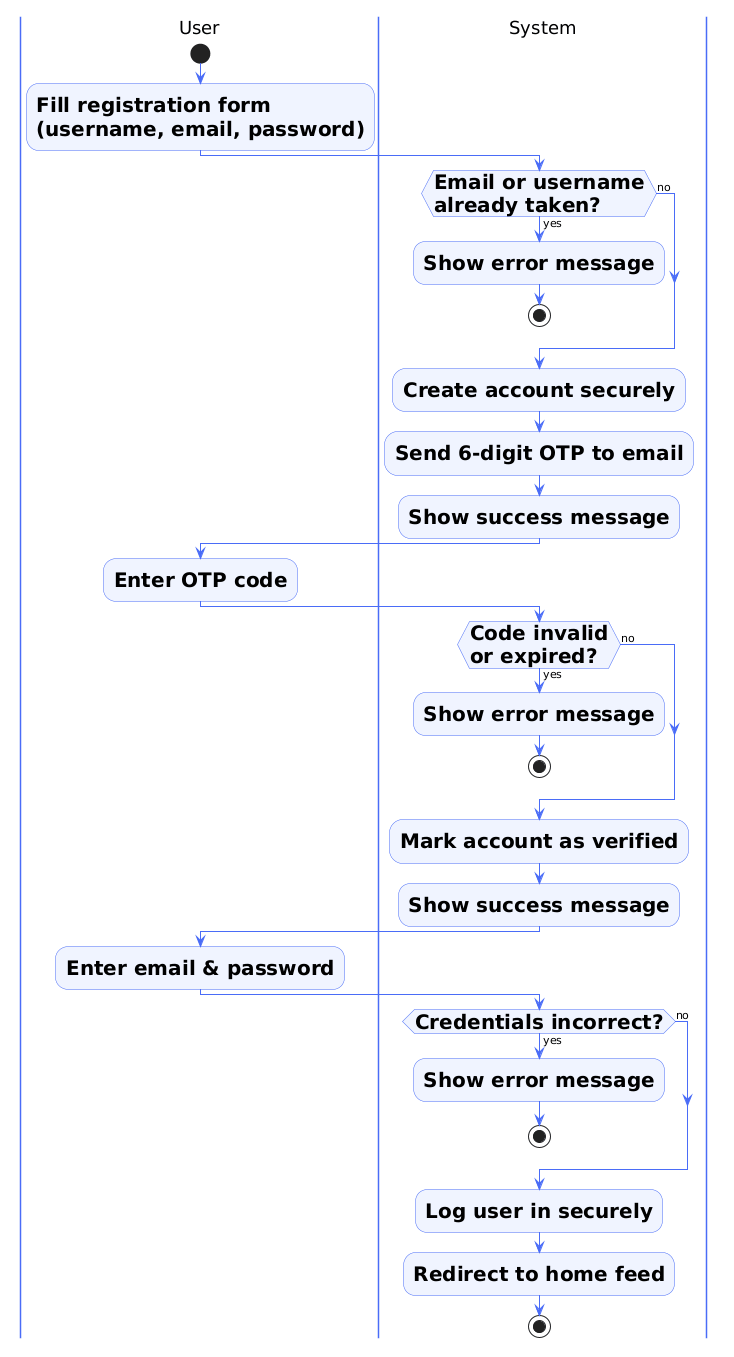
\includegraphics[width=0.92\linewidth,height=0.82\textheight,keepaspectratio]{images/image6.png}
  \caption{Authentication \& Account Management}
  \label{fig:3}
\end{figure}

\medskip\noindent\textbf{Feeds and Discovery:}\\[2pt]
\begin{figure}[H]
  \centering
  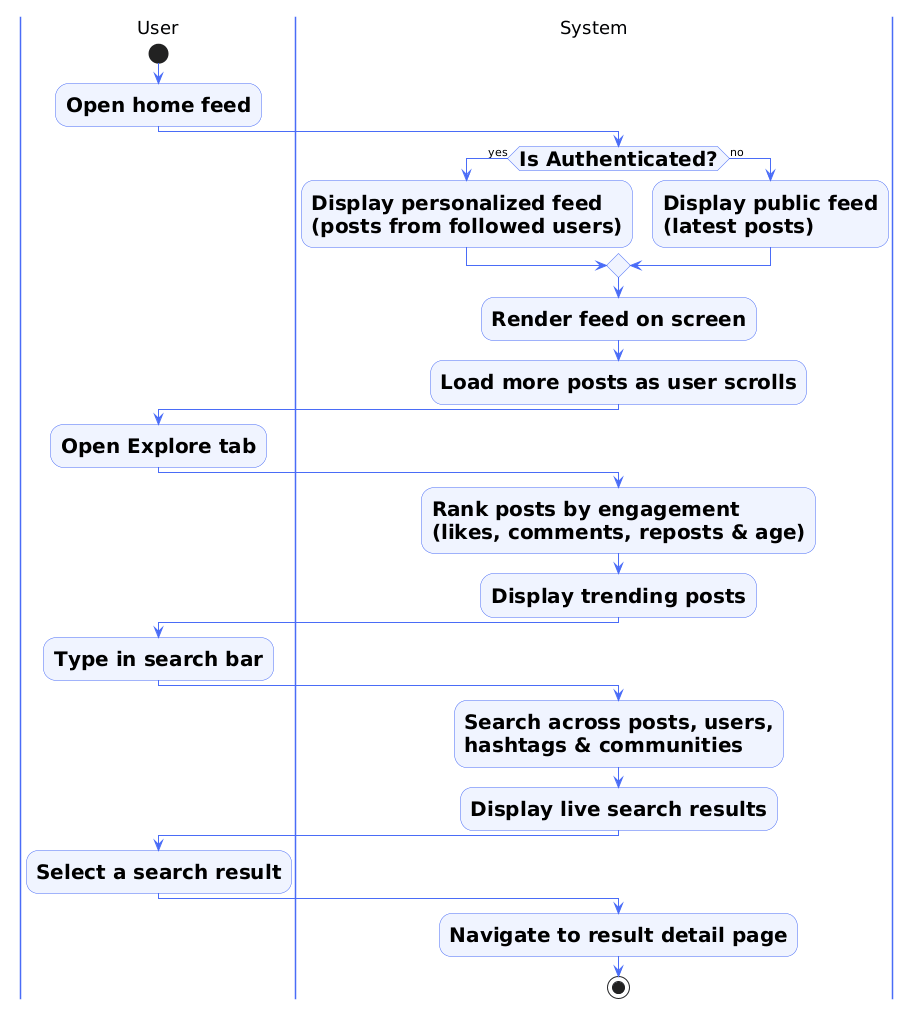
\includegraphics[width=0.92\linewidth,height=0.82\textheight,keepaspectratio]{images/image7.png}
  \caption{Feeds and Discovery}
  \label{fig:4}
\end{figure}

\medskip\noindent\textbf{Post Management:}\\[2pt]
\begin{figure}[H]
  \centering
  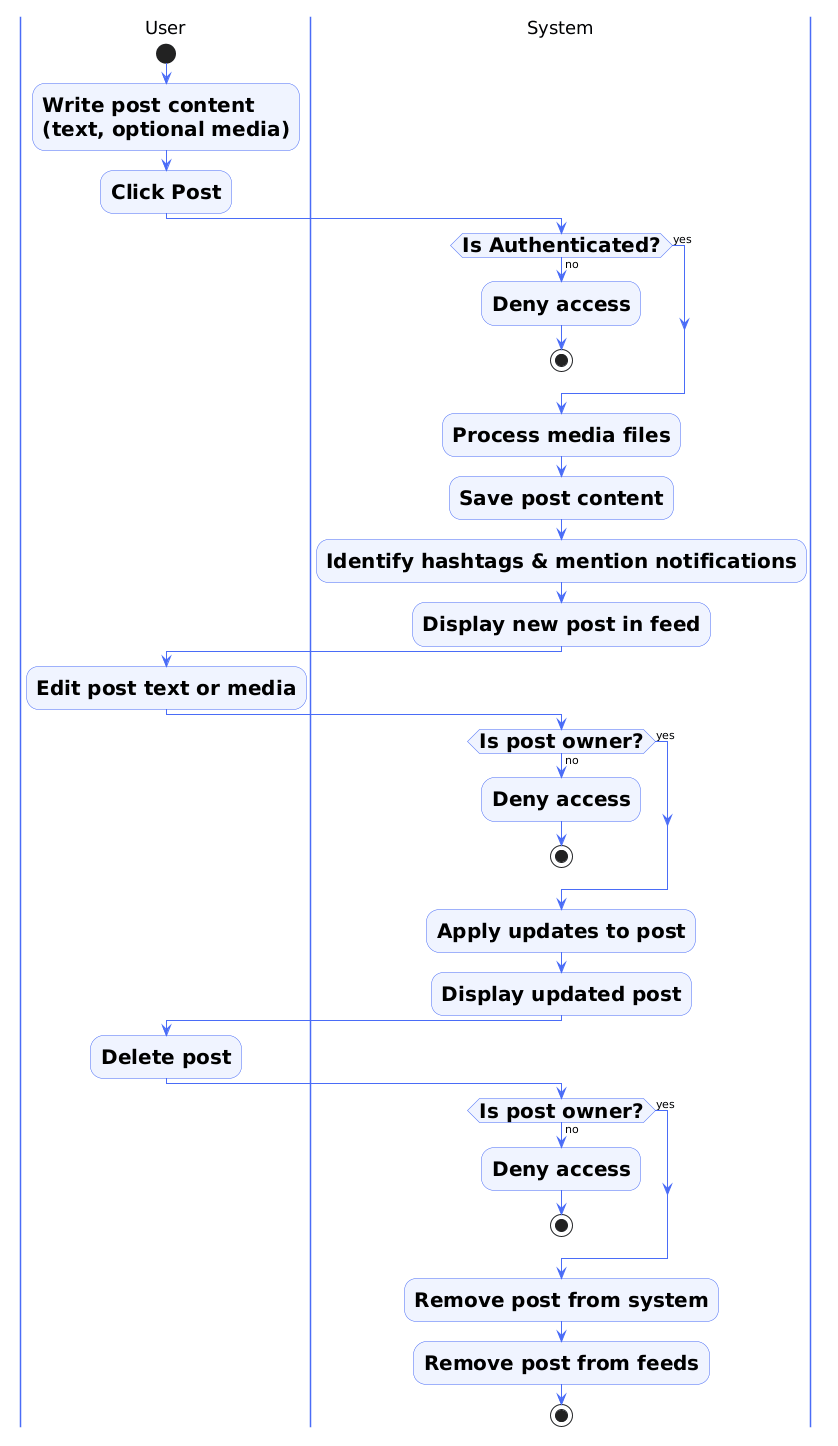
\includegraphics[width=0.92\linewidth,height=0.82\textheight,keepaspectratio]{images/image8.png}
  \caption{Post Management}
  \label{fig:5}
\end{figure}

\medskip\noindent\textbf{Post Interaction:}\\[2pt]
\begin{figure}[H]
  \centering
  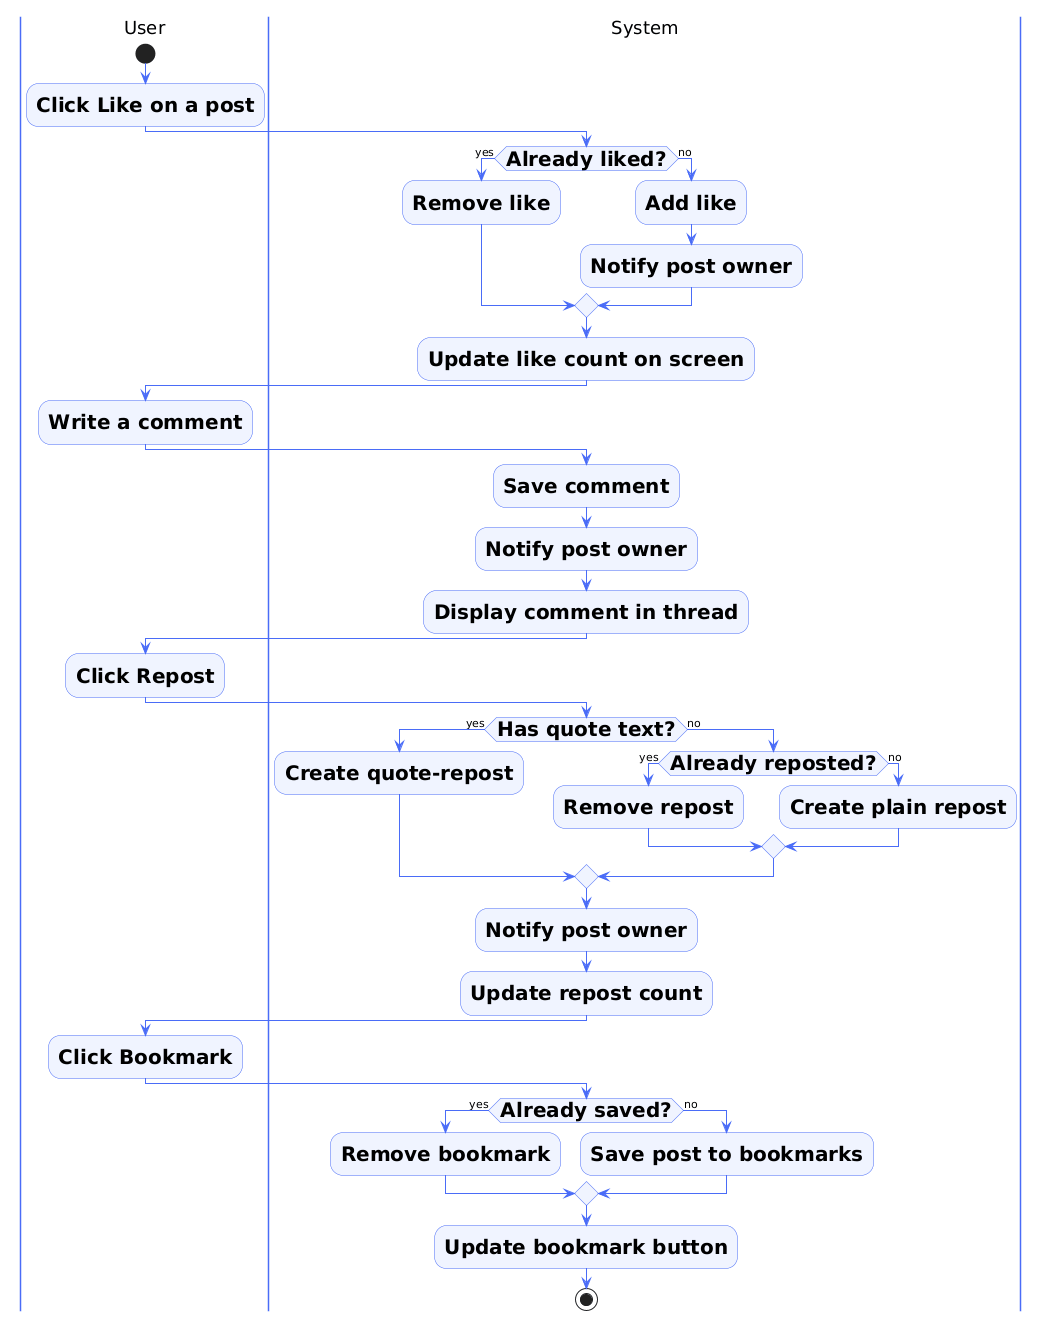
\includegraphics[width=0.92\linewidth,height=0.82\textheight,keepaspectratio]{images/image9.png}
  \caption{Post Interaction}
  \label{fig:6}
\end{figure}

\medskip\noindent\textbf{User Relationship Management:}\\[2pt]
\begin{figure}[H]
  \centering
  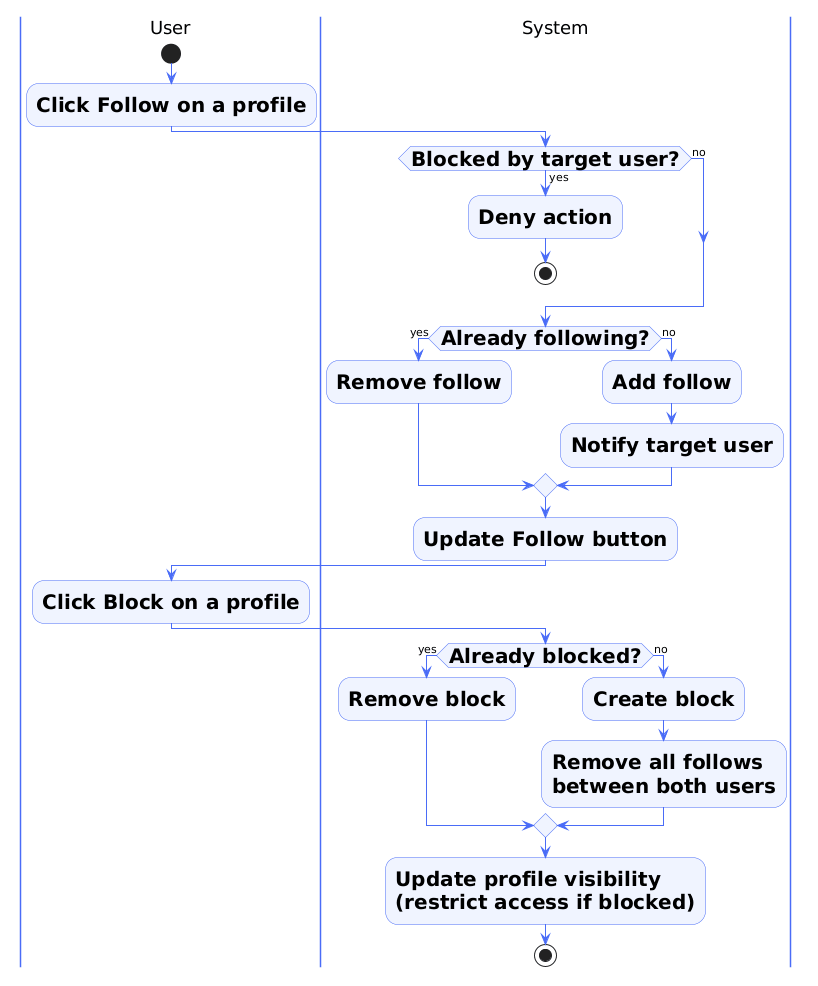
\includegraphics[width=0.92\linewidth,height=0.82\textheight,keepaspectratio]{images/image10.png}
  \caption{User Relationship Management}
  \label{fig:7}
\end{figure}

\medskip\noindent\textbf{User Profile Management:}\\[2pt]
\begin{figure}[H]
  \centering
  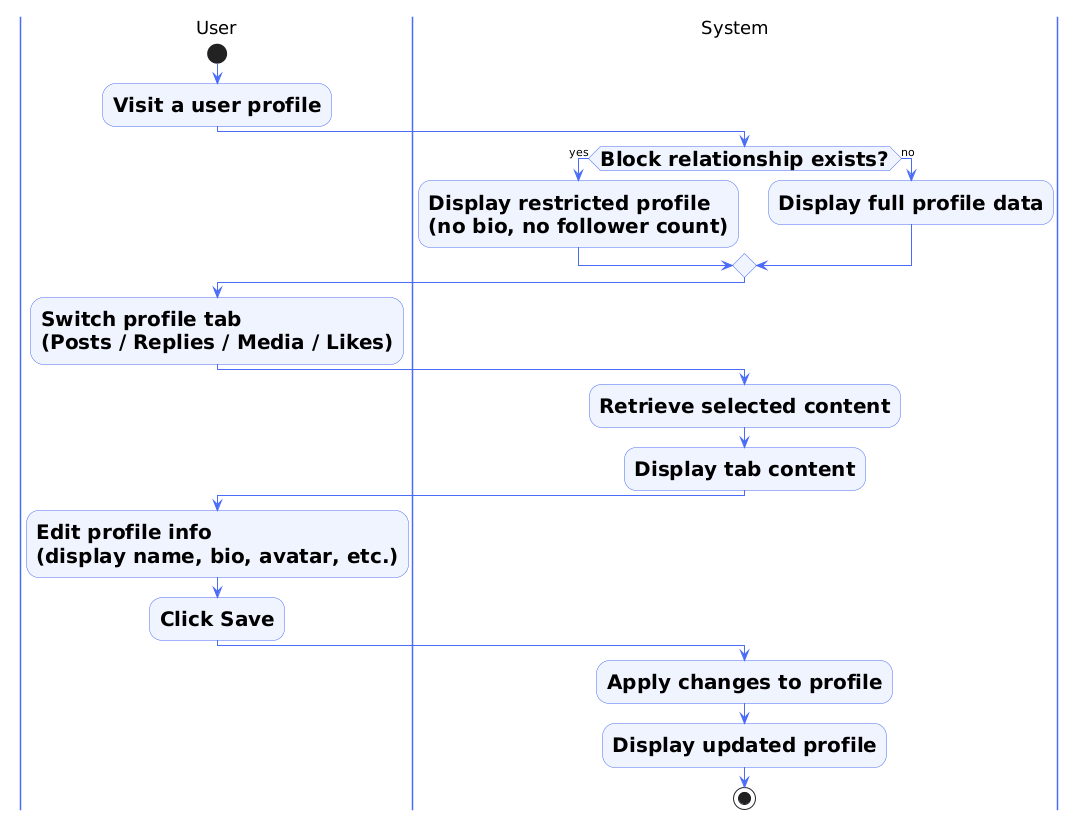
\includegraphics[width=0.92\linewidth,height=0.82\textheight,keepaspectratio]{images/image11.png}
  \caption{User Profile Management}
  \label{fig:8}
\end{figure}

\medskip\noindent\textbf{Direct Messaging:}\\[2pt]
\begin{figure}[H]
  \centering
  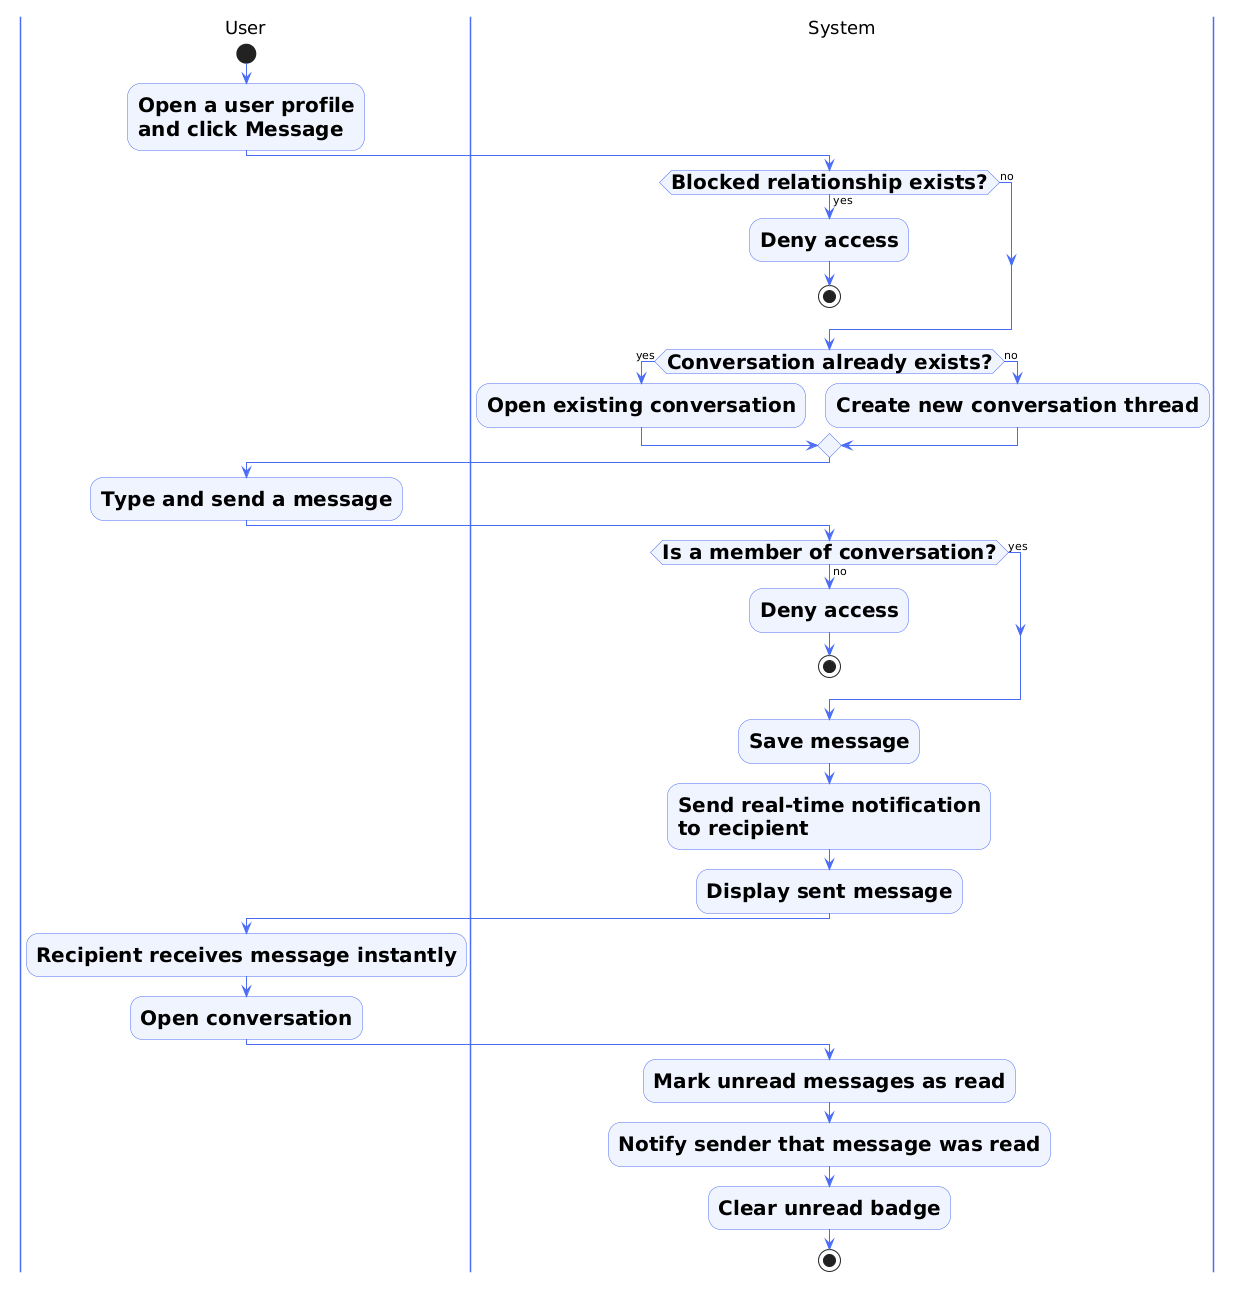
\includegraphics[width=0.92\linewidth,height=0.82\textheight,keepaspectratio]{images/image12.png}
  \caption{Direct Messaging}
  \label{fig:9}
\end{figure}

\medskip\noindent\textbf{Real-time Notifications:}\\[2pt]
\begin{figure}[H]
  \centering
  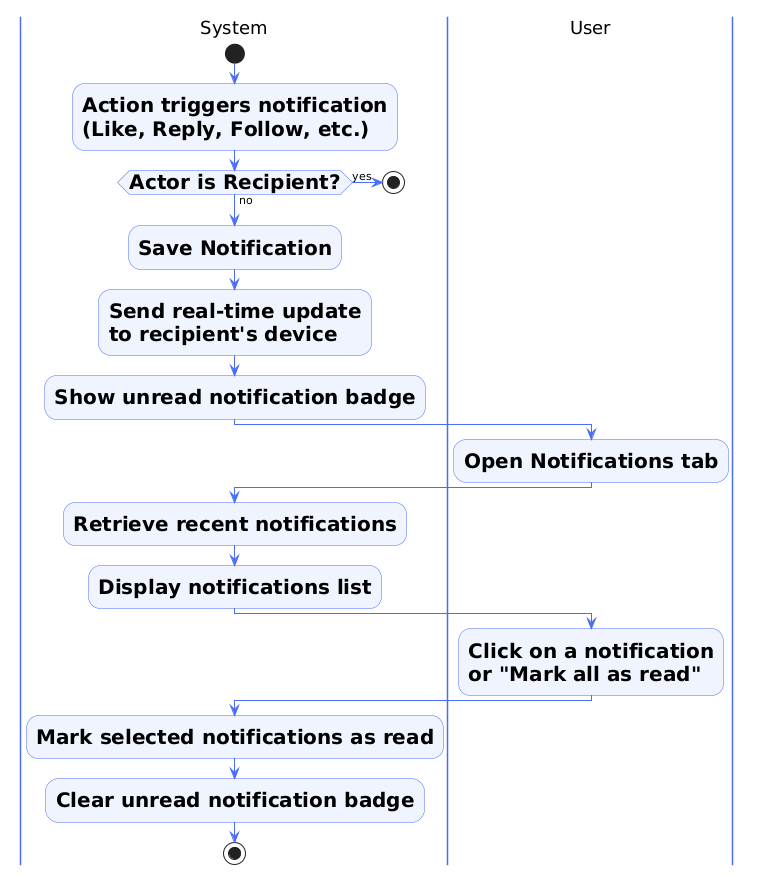
\includegraphics[width=0.92\linewidth,height=0.82\textheight,keepaspectratio]{images/image13.png}
  \caption{Real-time Notifications}
  \label{fig:10}
\end{figure}

\medskip\noindent\textbf{Community Management:}\\[2pt]
\begin{figure}[H]
  \centering
  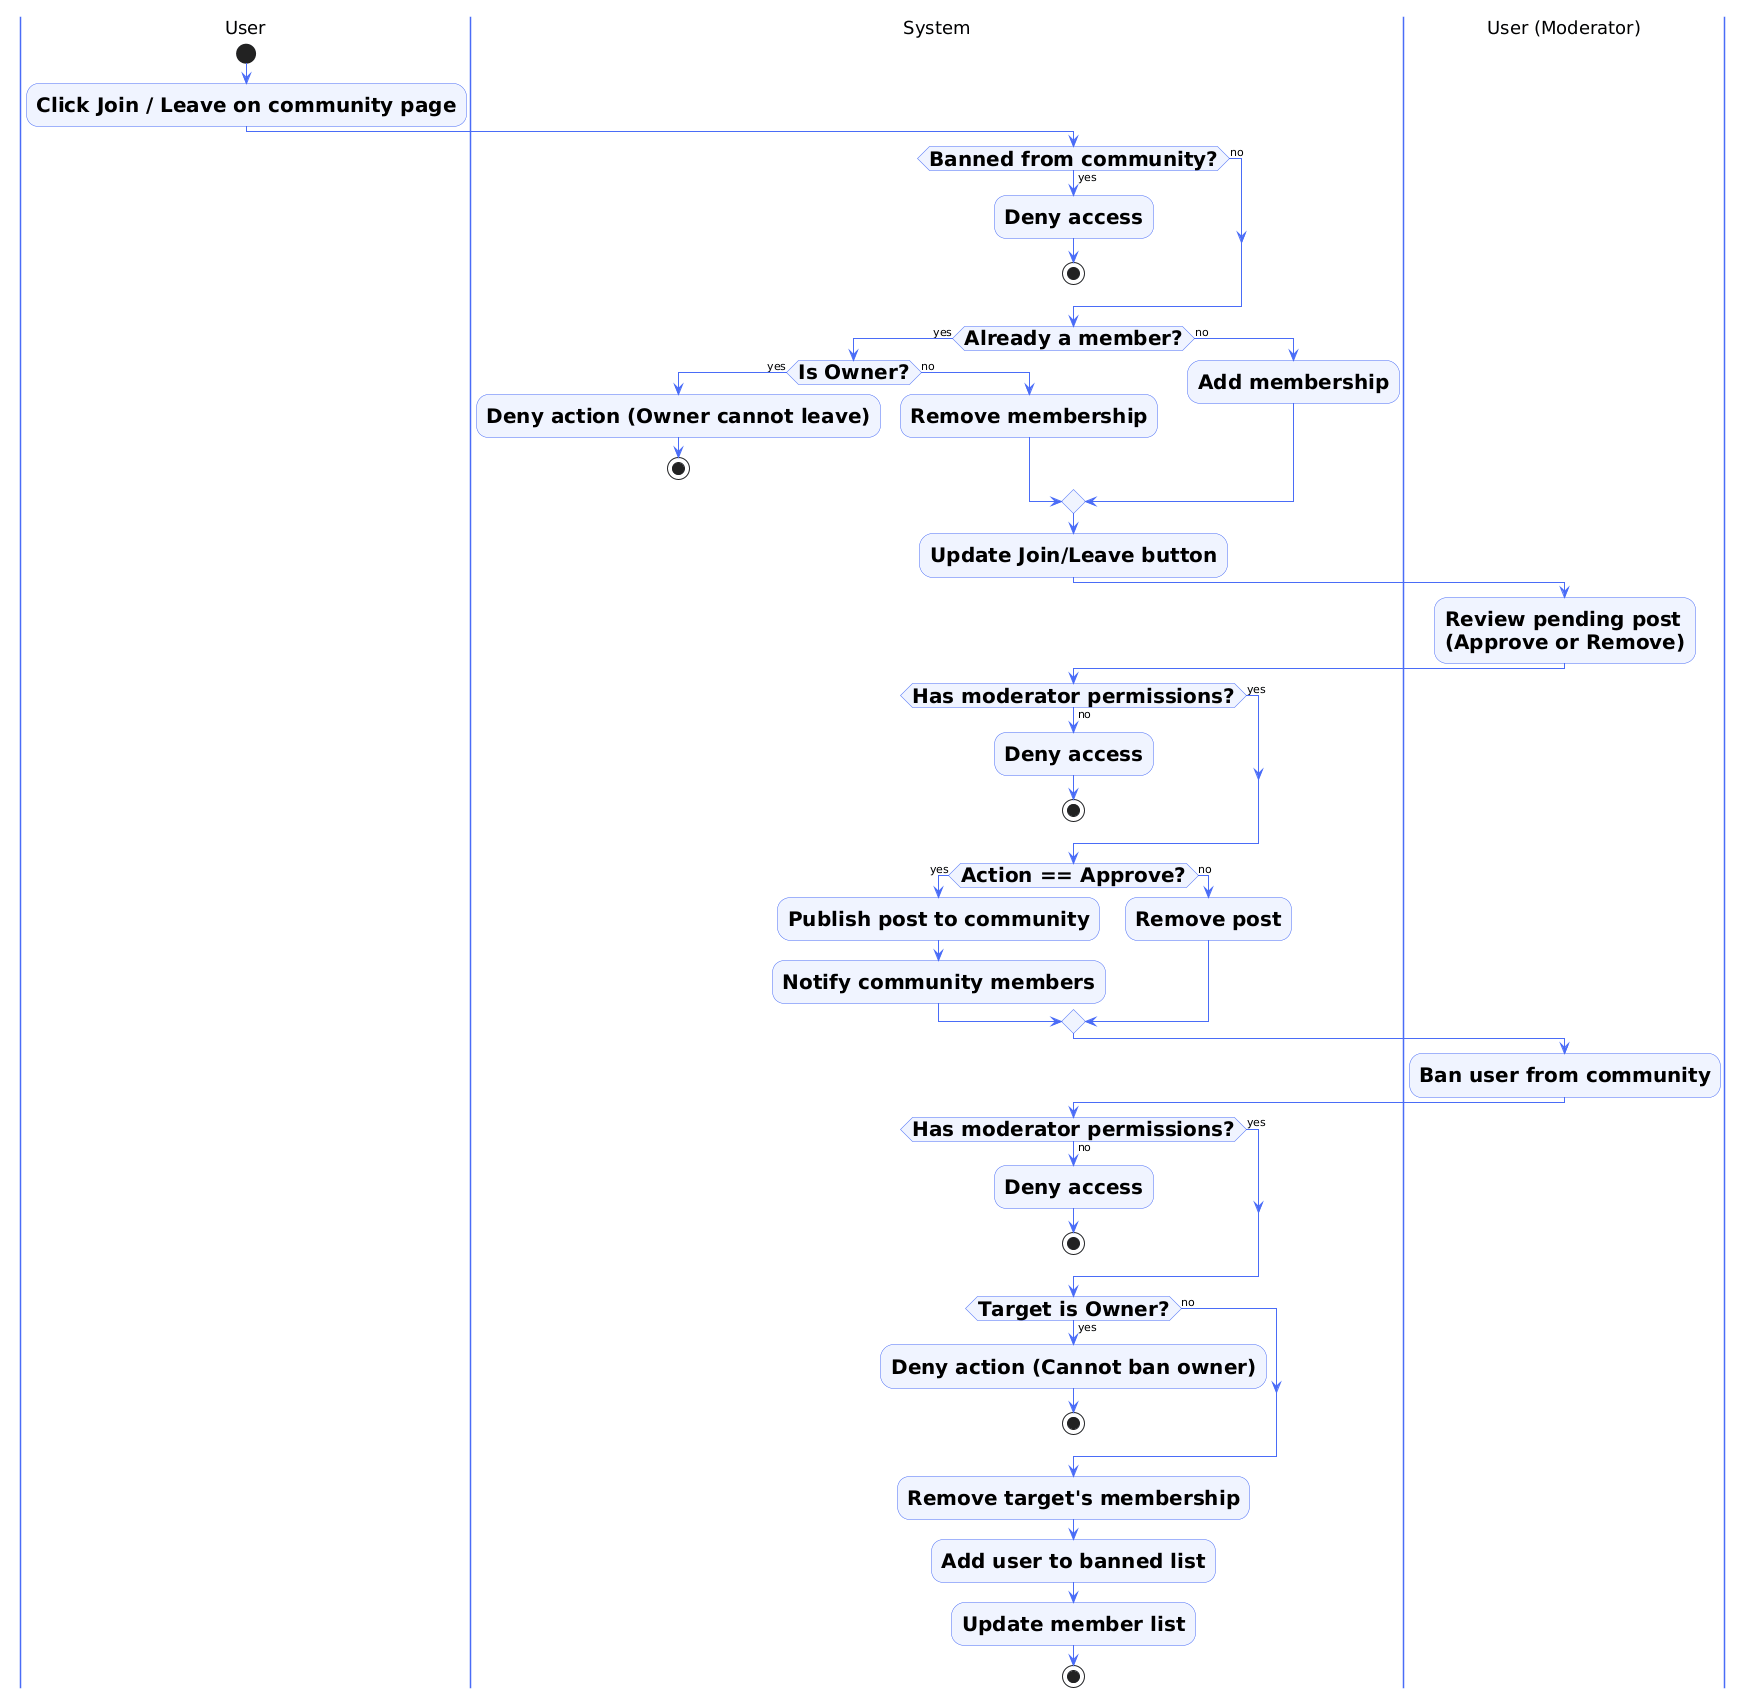
\includegraphics[width=0.92\linewidth,height=0.82\textheight,keepaspectratio]{images/image14.png}
  \caption{Community Management}
  \label{fig:11}
\end{figure}

\medskip\noindent\textbf{Administrative Moderation:}\\[2pt]
\begin{figure}[H]
  \centering
  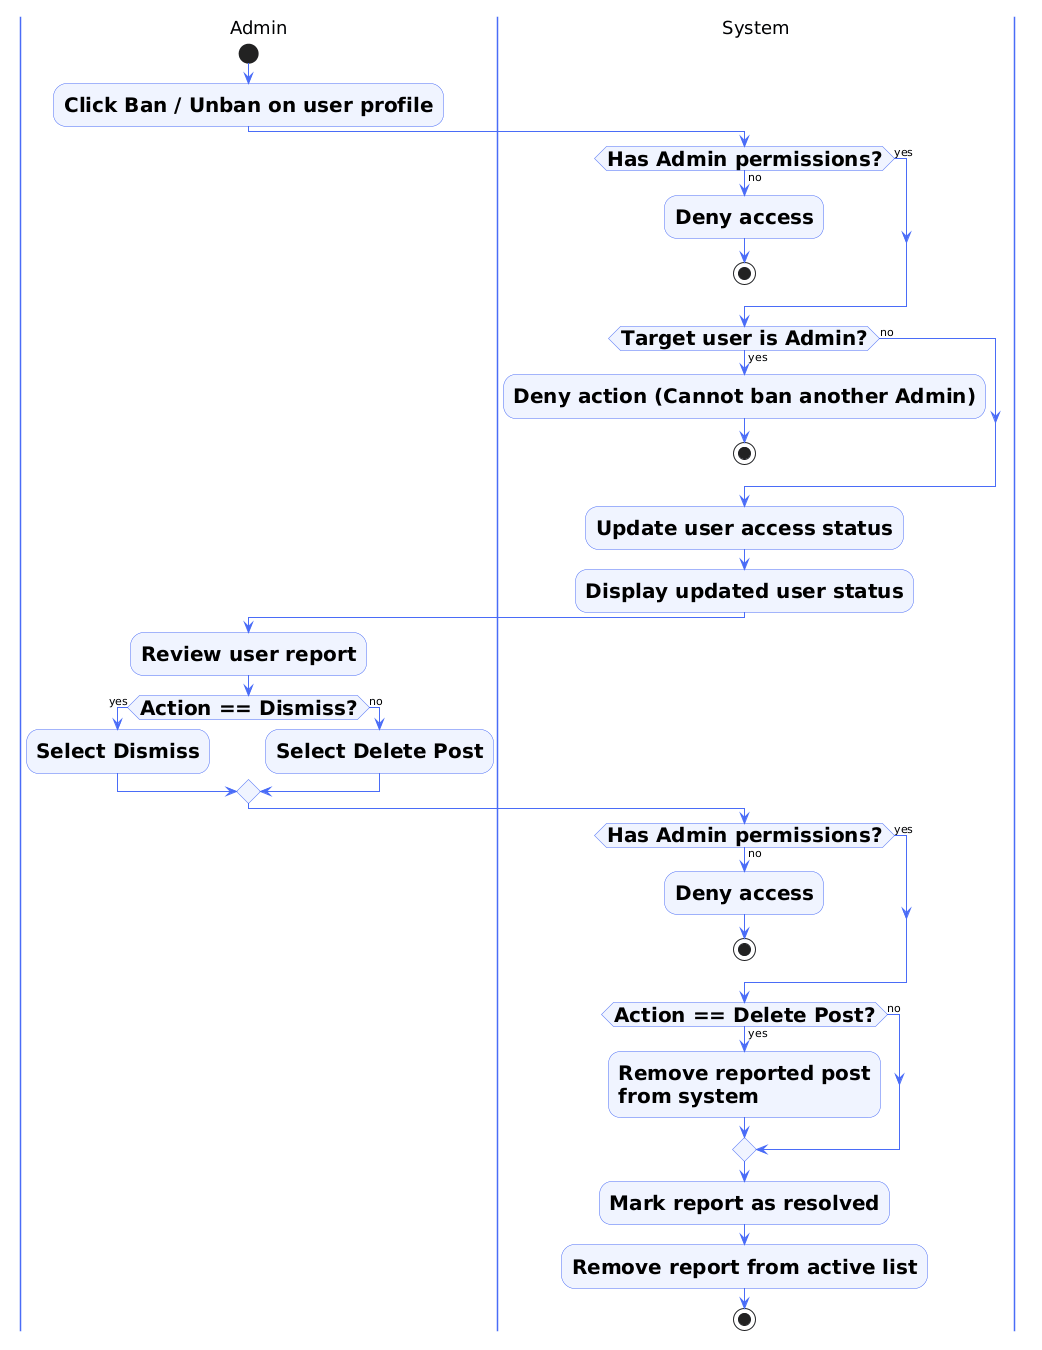
\includegraphics[width=0.92\linewidth,height=0.82\textheight,keepaspectratio]{images/image15.png}
  \caption{Administrative Moderation}
  \label{fig:12}
\end{figure}

\subsubsection{Entity Relationship Diagram:}
\begin{figure}[H]
  \centering
  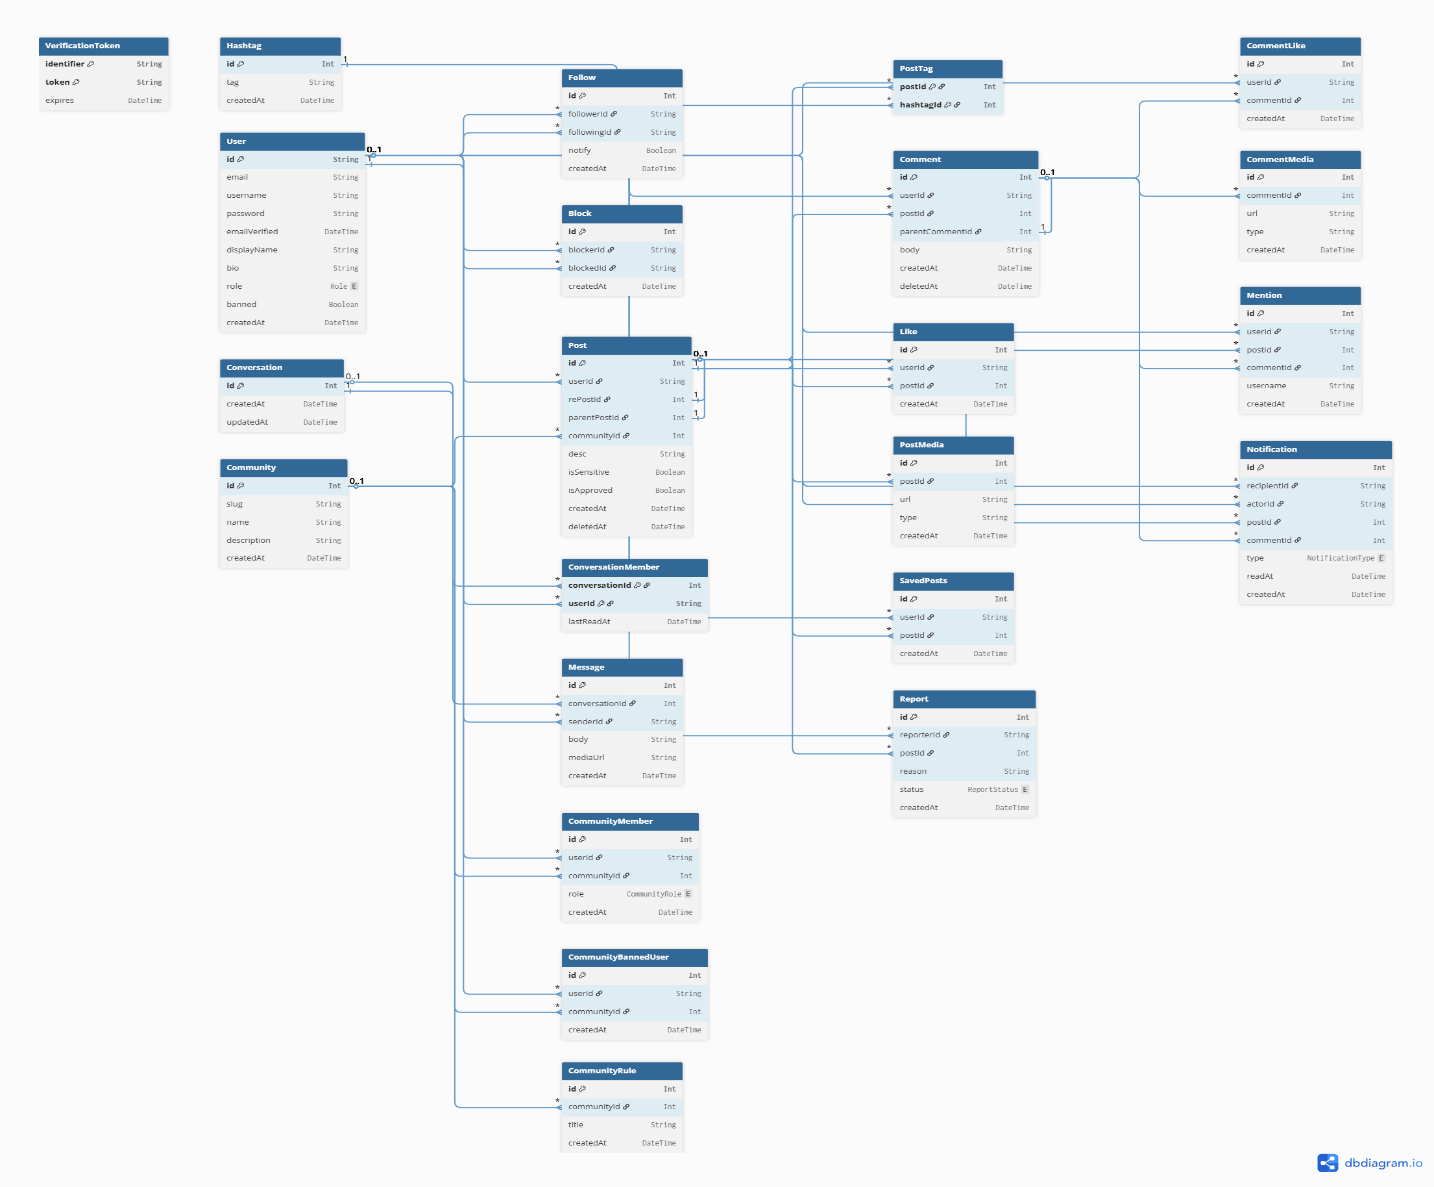
\includegraphics[width=0.92\linewidth,height=0.82\textheight,keepaspectratio]{images/image17.png}
  \caption{Entity Relationship Diagram}
  \label{fig:13}
\end{figure}

This section covers the all-database entities (tables) for the project. A more detailed and higher resolution version of the Entity Relationship Diagram is available in the Appendix section.

Summary:
\begin{enumerate}
  \item \textbf{Identity \& Access }\textbf{-Related Tables}
\end{enumerate}
\begin{figure}[H]
  \centering
  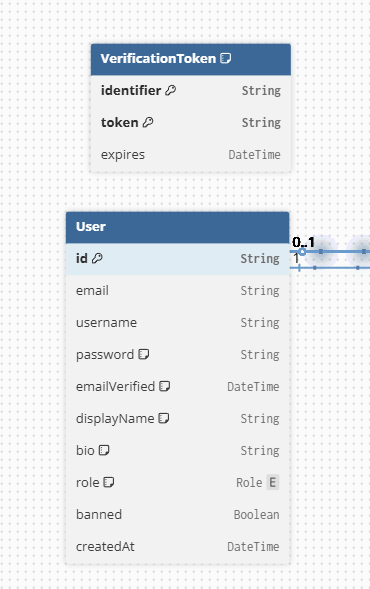
\includegraphics[width=0.92\linewidth,height=0.82\textheight,keepaspectratio]{images/image18.png}
  \caption{Identity \& Access -- Related Tables}
  \label{fig:14}
\end{figure}

\begin{longtable}{|p{0.45\linewidth}|p{0.45\linewidth}|}
\caption{Identity \& Access - Related Tables} \label{tab:17} \\
\hline
\textbf{\textbullet User  Description:~Core entity representing every platform account, storing identity, profile, and system-level access state.  Fields:}\newline id~(PK, String, cuid)\newline email~(String, unique)\newline username~(String, unique)\newline password~(String, nullable)\newline emailVerified~(DateTime, nullable)\newline displayName~(String, nullable)\newline bio~(String, nullable)\newline location~(String, nullable)\newline job~(String, nullable)\newline website~(String, nullable)\newline img~(String, nullable)\newline cover~(String, nullable)\newline role~(Enum: USER | ADMIN)\newline banned~(Boolean, default: false)\newline createdAt~/~updatedAt~(DateTime)\newline Relationships:\newline One-to-Many with interaction tables (Post, Comment, Like, etc.) & \textbf{\textbullet VerificationToken  Description:~Stores single-use OTP codes for email verification and password reset flows. Automatically deleted after use or expiry.  Fields:}\newline identifier~(PK, String) - e.g., "email-verify:user123"\newline token~(PK, String) - 6-digit OTP or UUID string\newline expires~(DateTime) - Expiration timestamp\newline Relationships:\newline One-to-Many with nearly all other tables (Post, Comment, Like, Follow, etc. \\
\hline
\endfirsthead
\multicolumn{2}{l}{\textit{(Continued from previous page)}} \\
\hline
\textbf{\textbullet User  Description:~Core entity representing every platform account, storing identity, profile, and system-level access state.  Fields:}\newline id~(PK, String, cuid)\newline email~(String, unique)\newline username~(String, unique)\newline password~(String, nullable)\newline emailVerified~(DateTime, nullable)\newline displayName~(String, nullable)\newline bio~(String, nullable)\newline location~(String, nullable)\newline job~(String, nullable)\newline website~(String, nullable)\newline img~(String, nullable)\newline cover~(String, nullable)\newline role~(Enum: USER | ADMIN)\newline banned~(Boolean, default: false)\newline createdAt~/~updatedAt~(DateTime)\newline Relationships:\newline One-to-Many with interaction tables (Post, Comment, Like, etc.) & \textbf{\textbullet VerificationToken  Description:~Stores single-use OTP codes for email verification and password reset flows. Automatically deleted after use or expiry.  Fields:}\newline identifier~(PK, String) - e.g., "email-verify:user123"\newline token~(PK, String) - 6-digit OTP or UUID string\newline expires~(DateTime) - Expiration timestamp\newline Relationships:\newline One-to-Many with nearly all other tables (Post, Comment, Like, Follow, etc. \\
\hline
\endhead
\hline \multicolumn{2}{r}{\textit{Continued on next page}} \\
\endfoot
\hline
\endlastfoot
\end{longtable}

\begin{enumerate}
  \item \textbf{Content }\textbf{-Related Table}\textbf{s}
\end{enumerate}
\begin{figure}[H]
  \centering
  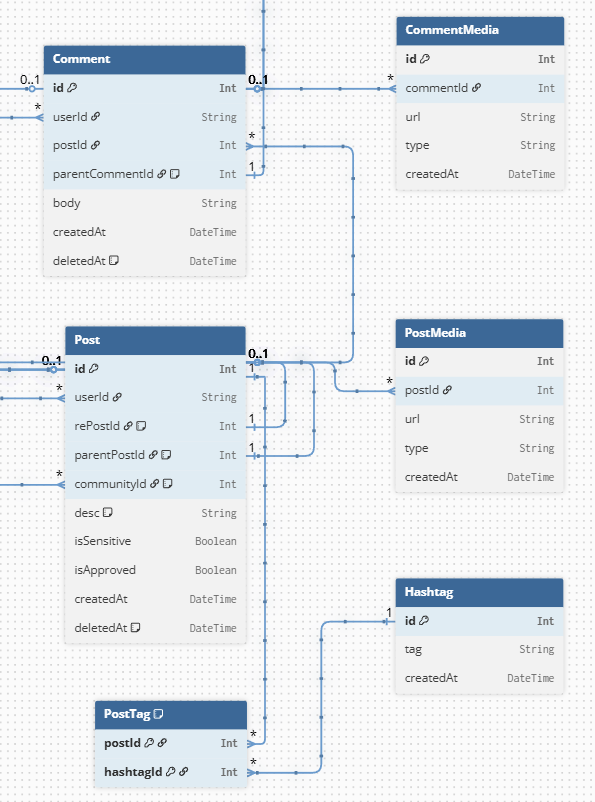
\includegraphics[width=0.92\linewidth,height=0.82\textheight,keepaspectratio]{images/image19.png}
  \caption{Content -- Related Tables}
  \label{fig:15}
\end{figure}

\begin{longtable}{|p{0.45\linewidth}|p{0.45\linewidth}|}
\caption{Content -Related Tables} \label{tab:18} \\
\hline
\textbf{\textbullet Post Description:~The backbone of the feed. Represents original post, repost, and through self-referencing belong community.}\newline Fields:\newline id~(PK, Int)\newline userId~(FK, String) - The author\newline communityId~(FK, Int, nullable)\newline desc~(String, nullable)\newline isSensitive~(Boolean\newline isApproved~(Boolean)\newline rePostId~(FK, Int, nullable)\newline parentPostId~(FK, Int, nullable) -\newline deletedAt~(DateTime, nullable)\newline Relationships:\newline Self-reference for reposts\newline Many-to-One with User, Community\newline One-to-Many with PostMedia, Comment, Like, SavedPosts, PostTag, Notification, Report, Mention & \textbf{\textbullet PostMedia Description:~Stores images/videos attached Post.}\newline Fields:\newline id (PK, Int)\newline postId (FK, Int)\newline url (String) CDN path (Cloudinary/S3)\newline type (String) --- "IMAGE" | "VIDEO" | "FILE"\newline width, height (Int, nullable) Used for layout rendering\newline createdAt (DateTime)\newline Relationships:\newline Many-to-One with~Post~(Cascade delete) \\
\hline
\endfirsthead
\multicolumn{2}{l}{\textit{(Continued from previous page)}} \\
\hline
\textbf{\textbullet Post Description:~The backbone of the feed. Represents original post, repost, and through self-referencing belong community.}\newline Fields:\newline id~(PK, Int)\newline userId~(FK, String) - The author\newline communityId~(FK, Int, nullable)\newline desc~(String, nullable)\newline isSensitive~(Boolean\newline isApproved~(Boolean)\newline rePostId~(FK, Int, nullable)\newline parentPostId~(FK, Int, nullable) -\newline deletedAt~(DateTime, nullable)\newline Relationships:\newline Self-reference for reposts\newline Many-to-One with User, Community\newline One-to-Many with PostMedia, Comment, Like, SavedPosts, PostTag, Notification, Report, Mention & \textbf{\textbullet PostMedia Description:~Stores images/videos attached Post.}\newline Fields:\newline id (PK, Int)\newline postId (FK, Int)\newline url (String) CDN path (Cloudinary/S3)\newline type (String) --- "IMAGE" | "VIDEO" | "FILE"\newline width, height (Int, nullable) Used for layout rendering\newline createdAt (DateTime)\newline Relationships:\newline Many-to-One with~Post~(Cascade delete) \\
\hline
\endhead
\hline \multicolumn{2}{r}{\textit{Continued on next page}} \\
\endfoot
\hline
\endlastfoot
\textbullet Comment Description:~Stores user replies to a Post. Fields:\newline id (PK, Int)\newline postId (FK, Int)\newline url (String) CDN path (Cloudinary/S3)\newline type (String) --- "IMAGE" | "VIDEO" | "FILE"\newline width, height (Int, nullable)\newline createdAt (DateTime)\newline Relationships:\newline Self-referencing nested comment tree\newline Many-to-One with User, Post\newline One-to-Many with CommentMedia, CommentLike, Mention, Notification & \textbullet CommentMedia Description:~File attachments inside comments. Fields:\newline id (PK, Int)\newline commentId (FK, Int)\newline url (String) CDN path\newline type (String) --- "IMAGE" | "VIDEO" | "FILE"\newline width, height (Int, nullable)\newline createdAt (DateTime)\newline Relationships:\newline Many-to-One with~Comment \\
\hline
\textbullet Hashtag Description:~Normalized registry of tags to serve the Trending feature. Fields:\newline id (PK, Int)\newline tag (String, unique) Lowercase tag string, e.g. "technology"\newline createdAt (DateTime)\newline Relationships:\newline One-to-Many with~PostTag & \textbullet PostTag Description:~Join table resolving the Many-to-Many relationship between Posts and Hashtags. Created/updated automatically when a post is submitted or edited. Fields:\newline postId~(PK, FK, Int)\newline hashtagId~(PK, FK, Int)\newline Relationships:\newline Composite Primary Key with 2 FKs. \\
\hline
\end{longtable}

\begin{enumerate}
  \item \textbf{Social Engagement}\textbf{ Tables}
\end{enumerate}
\begin{figure}[H]
  \centering
  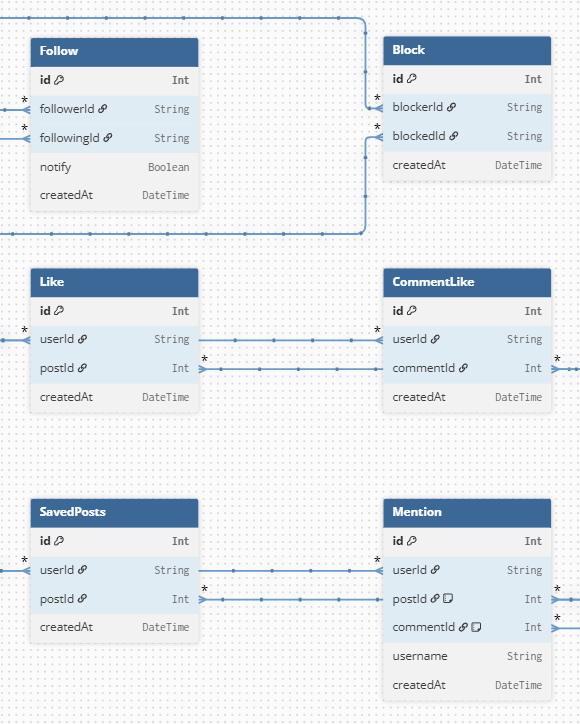
\includegraphics[width=0.92\linewidth,height=0.82\textheight,keepaspectratio]{images/image20.png}
  \caption{Social Engagement -- Related Tables}
  \label{fig:16}
\end{figure}

\begin{longtable}{|p{0.45\linewidth}|p{0.45\linewidth}|}
\caption{Social Engagement -- Related Tables} \label{tab:19} \\
\hline
\textbf{\textbullet  Follow Description:~Directed social graph edge. Determines which users appear in the personalized home feed of the follower. Fields:}\newline id (PK, Int)\newline followerId (FK, String)\newline followingId (FK, String)\newline notify (Boolean, default: false) Push notification preference for this specific follow\newline createdAt (DateTime)\newline Relationships:\newline Many-to-One with User twice (follower and following sides) & \textbf{\textbullet Block  Description:~Mutual blacklist between two users. Prevents all interactions (follow, message, view posts). Automatically removes existing follows between both parties. Fields:}\newline id (PK, Int)\newline blockerId (FK, String) --- The user initiating the block\newline blockedId (FK, String) --- The user being blocked\newline createdAt (DateTime)\newline Relationships:\newline Many-to-One with User twice.\newline Unique constraint on [blockerId, blockedId]. \\
\hline
\endfirsthead
\multicolumn{2}{l}{\textit{(Continued from previous page)}} \\
\hline
\textbf{\textbullet  Follow Description:~Directed social graph edge. Determines which users appear in the personalized home feed of the follower. Fields:}\newline id (PK, Int)\newline followerId (FK, String)\newline followingId (FK, String)\newline notify (Boolean, default: false) Push notification preference for this specific follow\newline createdAt (DateTime)\newline Relationships:\newline Many-to-One with User twice (follower and following sides) & \textbf{\textbullet Block  Description:~Mutual blacklist between two users. Prevents all interactions (follow, message, view posts). Automatically removes existing follows between both parties. Fields:}\newline id (PK, Int)\newline blockerId (FK, String) --- The user initiating the block\newline blockedId (FK, String) --- The user being blocked\newline createdAt (DateTime)\newline Relationships:\newline Many-to-One with User twice.\newline Unique constraint on [blockerId, blockedId]. \\
\hline
\endhead
\hline \multicolumn{2}{r}{\textit{Continued on next page}} \\
\endfoot
\hline
\endlastfoot
\textbullet   Like Description:~Records a User's "like" reaction on a Post. Triggers a LIKE notification to the post author. Fields:\newline id (PK, Int)\newline userId (FK, String)\newline postId (FK, Int)\newline createdAt (DateTime)\newline Relationships:\newline Many-to-One with User, Post & \textbullet  CommentLike\newline Description: Records a User's "like" reaction on a Comment. Unique constraint prevents double-liking.\newline Fields:\newline id (PK, Int)\newline userId (FK, String)\newline commentId (FK, Int)\newline createdAt (DateTime)\newline Relationships:\newline Many-to-One with User, Comment (Cascade delete)\newline Unique constraint on [userId, commentId] \\
\hline
\textbullet  SavedPosts\newline Description: User's personal bookmark list. Posts saved here appear in the /bookmarks.\newline Fields:\newline id (PK, Int)\newline userId (FK, String)\newline postId (FK, Int)\newline createdAt (DateTime)\newline Relationships:\newline Many-to-One with User, Post & \textbullet  Mention\newline Description: Records every @username tag inside a post or comment body. Parsed automatically on create/edit. Triggers a MENTION notification to the tagged user.\newline Fields:\newline id (PK, Int)\newline userId (FK, String)\newline username (String)\newline postId (FK, Int, nullable)\newline commentId (FK, Int, nullable)\newline createdAt (DateTime)\newline Relationships:\newline Many-to-One with User, Post, Comment (Cascade delete) \\
\hline
\end{longtable}

\begin{enumerate}
  \item \textbf{Community \& Moderation}\textbf{ Tables}
\end{enumerate}
\begin{figure}[H]
  \centering
  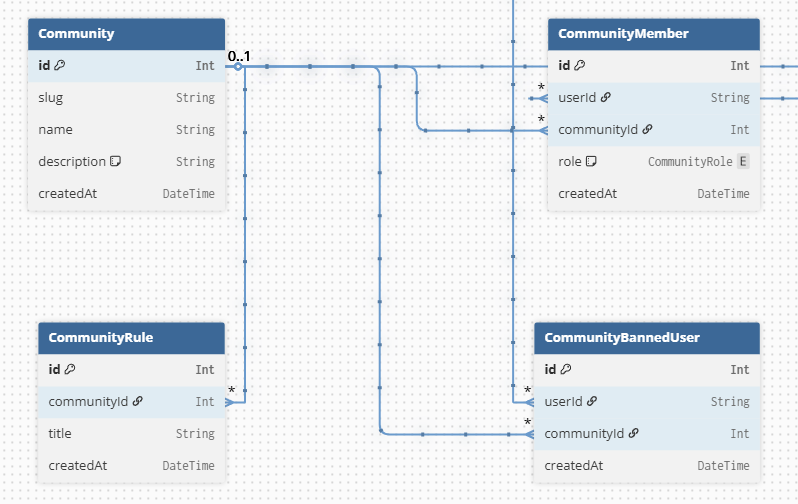
\includegraphics[width=0.92\linewidth,height=0.82\textheight,keepaspectratio]{images/image21.png}
  \caption{Community \& Moderation - Related Tables}
  \label{fig:17}
\end{figure}

\begin{longtable}{|p{0.45\linewidth}|p{0.45\linewidth}|}
\caption{Community \& Moderation Tables} \label{tab:20} \\
\hline
\textbf{\textbullet       Community Description:~Represents a Sub-reddit style group, a shared space for members with common interests. Fields:}\newline id (PK, Int)\newline slug (String, unique) URL identifier, e.g. breadit.com/c/technology\newline name (String) Display name\newline description (String, nullable)\newline img (String, nullable)\newline cover (String, nullable)\newline createdAt / updatedAt (DateTime)\newline Relationships:\newline One-to-Many with Post, Member, Rule, BannedUser & \textbf{CommunityMember Description:~Unique Constraint: 1 User can join a specific community only once.}\newline Fields:\newline id (PK, Int)\newline userId (FK, String)\newline communityId (FK, Int)\newline role (Enum: MEMBER | MOD | OWNER, default: MEMBER)\newline createdAt (DateTime)\newline Relationships:\newline Many-to-One with User, Community\newline Unique constraint on [userId, communityId] one role per user per community \\
\hline
\endfirsthead
\multicolumn{2}{l}{\textit{(Continued from previous page)}} \\
\hline
\textbf{\textbullet       Community Description:~Represents a Sub-reddit style group, a shared space for members with common interests. Fields:}\newline id (PK, Int)\newline slug (String, unique) URL identifier, e.g. breadit.com/c/technology\newline name (String) Display name\newline description (String, nullable)\newline img (String, nullable)\newline cover (String, nullable)\newline createdAt / updatedAt (DateTime)\newline Relationships:\newline One-to-Many with Post, Member, Rule, BannedUser & \textbf{CommunityMember Description:~Unique Constraint: 1 User can join a specific community only once.}\newline Fields:\newline id (PK, Int)\newline userId (FK, String)\newline communityId (FK, Int)\newline role (Enum: MEMBER | MOD | OWNER, default: MEMBER)\newline createdAt (DateTime)\newline Relationships:\newline Many-to-One with User, Community\newline Unique constraint on [userId, communityId] one role per user per community \\
\hline
\endhead
\hline \multicolumn{2}{r}{\textit{Continued on next page}} \\
\endfoot
\hline
\endlastfoot
\textbullet         CommunityRule Description:~Custom rules and regulations set by Community Admins. Fields:\newline id (PK, Int)\newline communityId (FK, Int)\newline title (String) - Rule headline\newline Relationships:\newline Many-to-One with Community & \textbullet  CommunityBannedUser Description:~Blacklist for individual Communities, enforced by local Moderators. Fields:\newline id~(PK, Int)\newline reason~(String, nullable) - Ban reason\newline userId~(FK, String) - The banned user\newline communityId~(FK, Int)\newline Relationships:\newline Many-to-One with User, Community\newline Unique [userId, communityId] \\
\hline
\end{longtable}

\begin{enumerate}
  \item \textbf{Communication }\textbf{Tables}
\end{enumerate}
\begin{figure}[H]
  \centering
  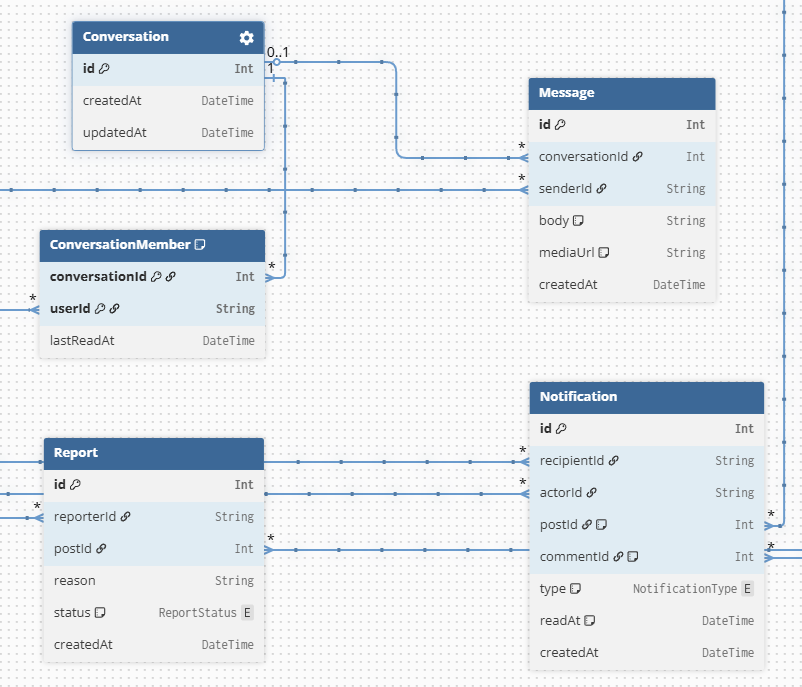
\includegraphics[width=0.92\linewidth,height=0.82\textheight,keepaspectratio]{images/image22.png}
  \caption{Communication -- Related Tables}
  \label{fig:18}
\end{figure}

\begin{longtable}{|p{0.45\linewidth}|p{0.45\linewidth}|}
\caption{Communication Tables} \label{tab:21} \\
\hline
\textbf{\textbullet  Conversation}\newline Description: Represents a single 1-to-1 Direct Message thread between two users. A conversation is created once and reused for all subsequent messages between the same pair.\newline Fields:\newline id (PK, Int)\newline createdAt (DateTime)\newline updatedAt (DateTime) Bumped on every new message; used to sort inbox by latest activity\newline Relationships:\newline One-to-Many with ConversationMember, Message & \textbf{\textbullet  ConversationMember}\newline Description: Junction table linking Users to Conversations. Tracks each participant's last-read timestamp, which powers the unread message badge count.\newline Fields:\newline conversationId (PK, FK, Int)\newline userId (PK, FK, String)\newline lastReadAt (DateTime, default: now()) Messages newer than this are considered "unread"\newline Relationships:\newline Composite PK ensures a user appears only once per conversation.\newline Many-to-One to Conversation, User \\
\hline
\endfirsthead
\multicolumn{2}{l}{\textit{(Continued from previous page)}} \\
\hline
\textbf{\textbullet  Conversation}\newline Description: Represents a single 1-to-1 Direct Message thread between two users. A conversation is created once and reused for all subsequent messages between the same pair.\newline Fields:\newline id (PK, Int)\newline createdAt (DateTime)\newline updatedAt (DateTime) Bumped on every new message; used to sort inbox by latest activity\newline Relationships:\newline One-to-Many with ConversationMember, Message & \textbf{\textbullet  ConversationMember}\newline Description: Junction table linking Users to Conversations. Tracks each participant's last-read timestamp, which powers the unread message badge count.\newline Fields:\newline conversationId (PK, FK, Int)\newline userId (PK, FK, String)\newline lastReadAt (DateTime, default: now()) Messages newer than this are considered "unread"\newline Relationships:\newline Composite PK ensures a user appears only once per conversation.\newline Many-to-One to Conversation, User \\
\hline
\endhead
\hline \multicolumn{2}{r}{\textit{Continued on next page}} \\
\endfoot
\hline
\endlastfoot
\textbullet  Message\newline Description: Individual message sent within a Conversation. Delivered in real-time via Socket.IO. Supports text and media attachments.\newline Fields:\newline id (PK, Int)\newline conversationId (FK, Int)\newline senderId (FK, String)\newline body (String, nullable, max 1000) Text content\newline mediaUrl (String, nullable) Image/file attachment URL\newline createdAt (DateTime)\newline Relationships:\newline Many-to-One with Conversation, User & \textbullet  Notification\newline Description: System-generated alert delivered to a recipient user when a relevant action occurs. Pushed in real-time via Socket.IO and persisted for the inbox view.\newline Fields:\newline id (PK, Int)\newline recipientId (FK, String)\newline actorId (FK, String)\newline type (Enum: LIKE | REPLY | REPOST | FOLLOW | MENTION | COMMUNITY\_POST | COMMUNITY\_NEW\_POST | COMMUNITY\_MOD\_ADDED | REPORT)\newline postId (FK, Int, nullable)\newline commentId (FK, Int, nullable)\newline readAt (DateTime, nullable)\newline createdAt (DateTime)\newline Relationships:\newline Many-to-One with User (recipient + actor), Post, Comment \\
\hline
\textbullet  Report\newline Description: Content flagging system. Any user can submit a report against a Post. System Admins review the report queue\newline Fields:\newline id (PK, Int)\newline reporterId (FK, String) --- The user who submitted the report\newline postId (FK, Int) --- The flagged post\newline reason (String) Report reason text (e.g., "Spam", "Hate speech")\newline status (Enum: OPEN | CLOSED, default: OPEN)\newline createdAt (DateTime)\newline Relationships:\newline Many-to-One with User (reporter), Post &  \\
\hline
\end{longtable}


\subsubsection{Class Diagram:}
\begin{figure}[H]
  \centering
  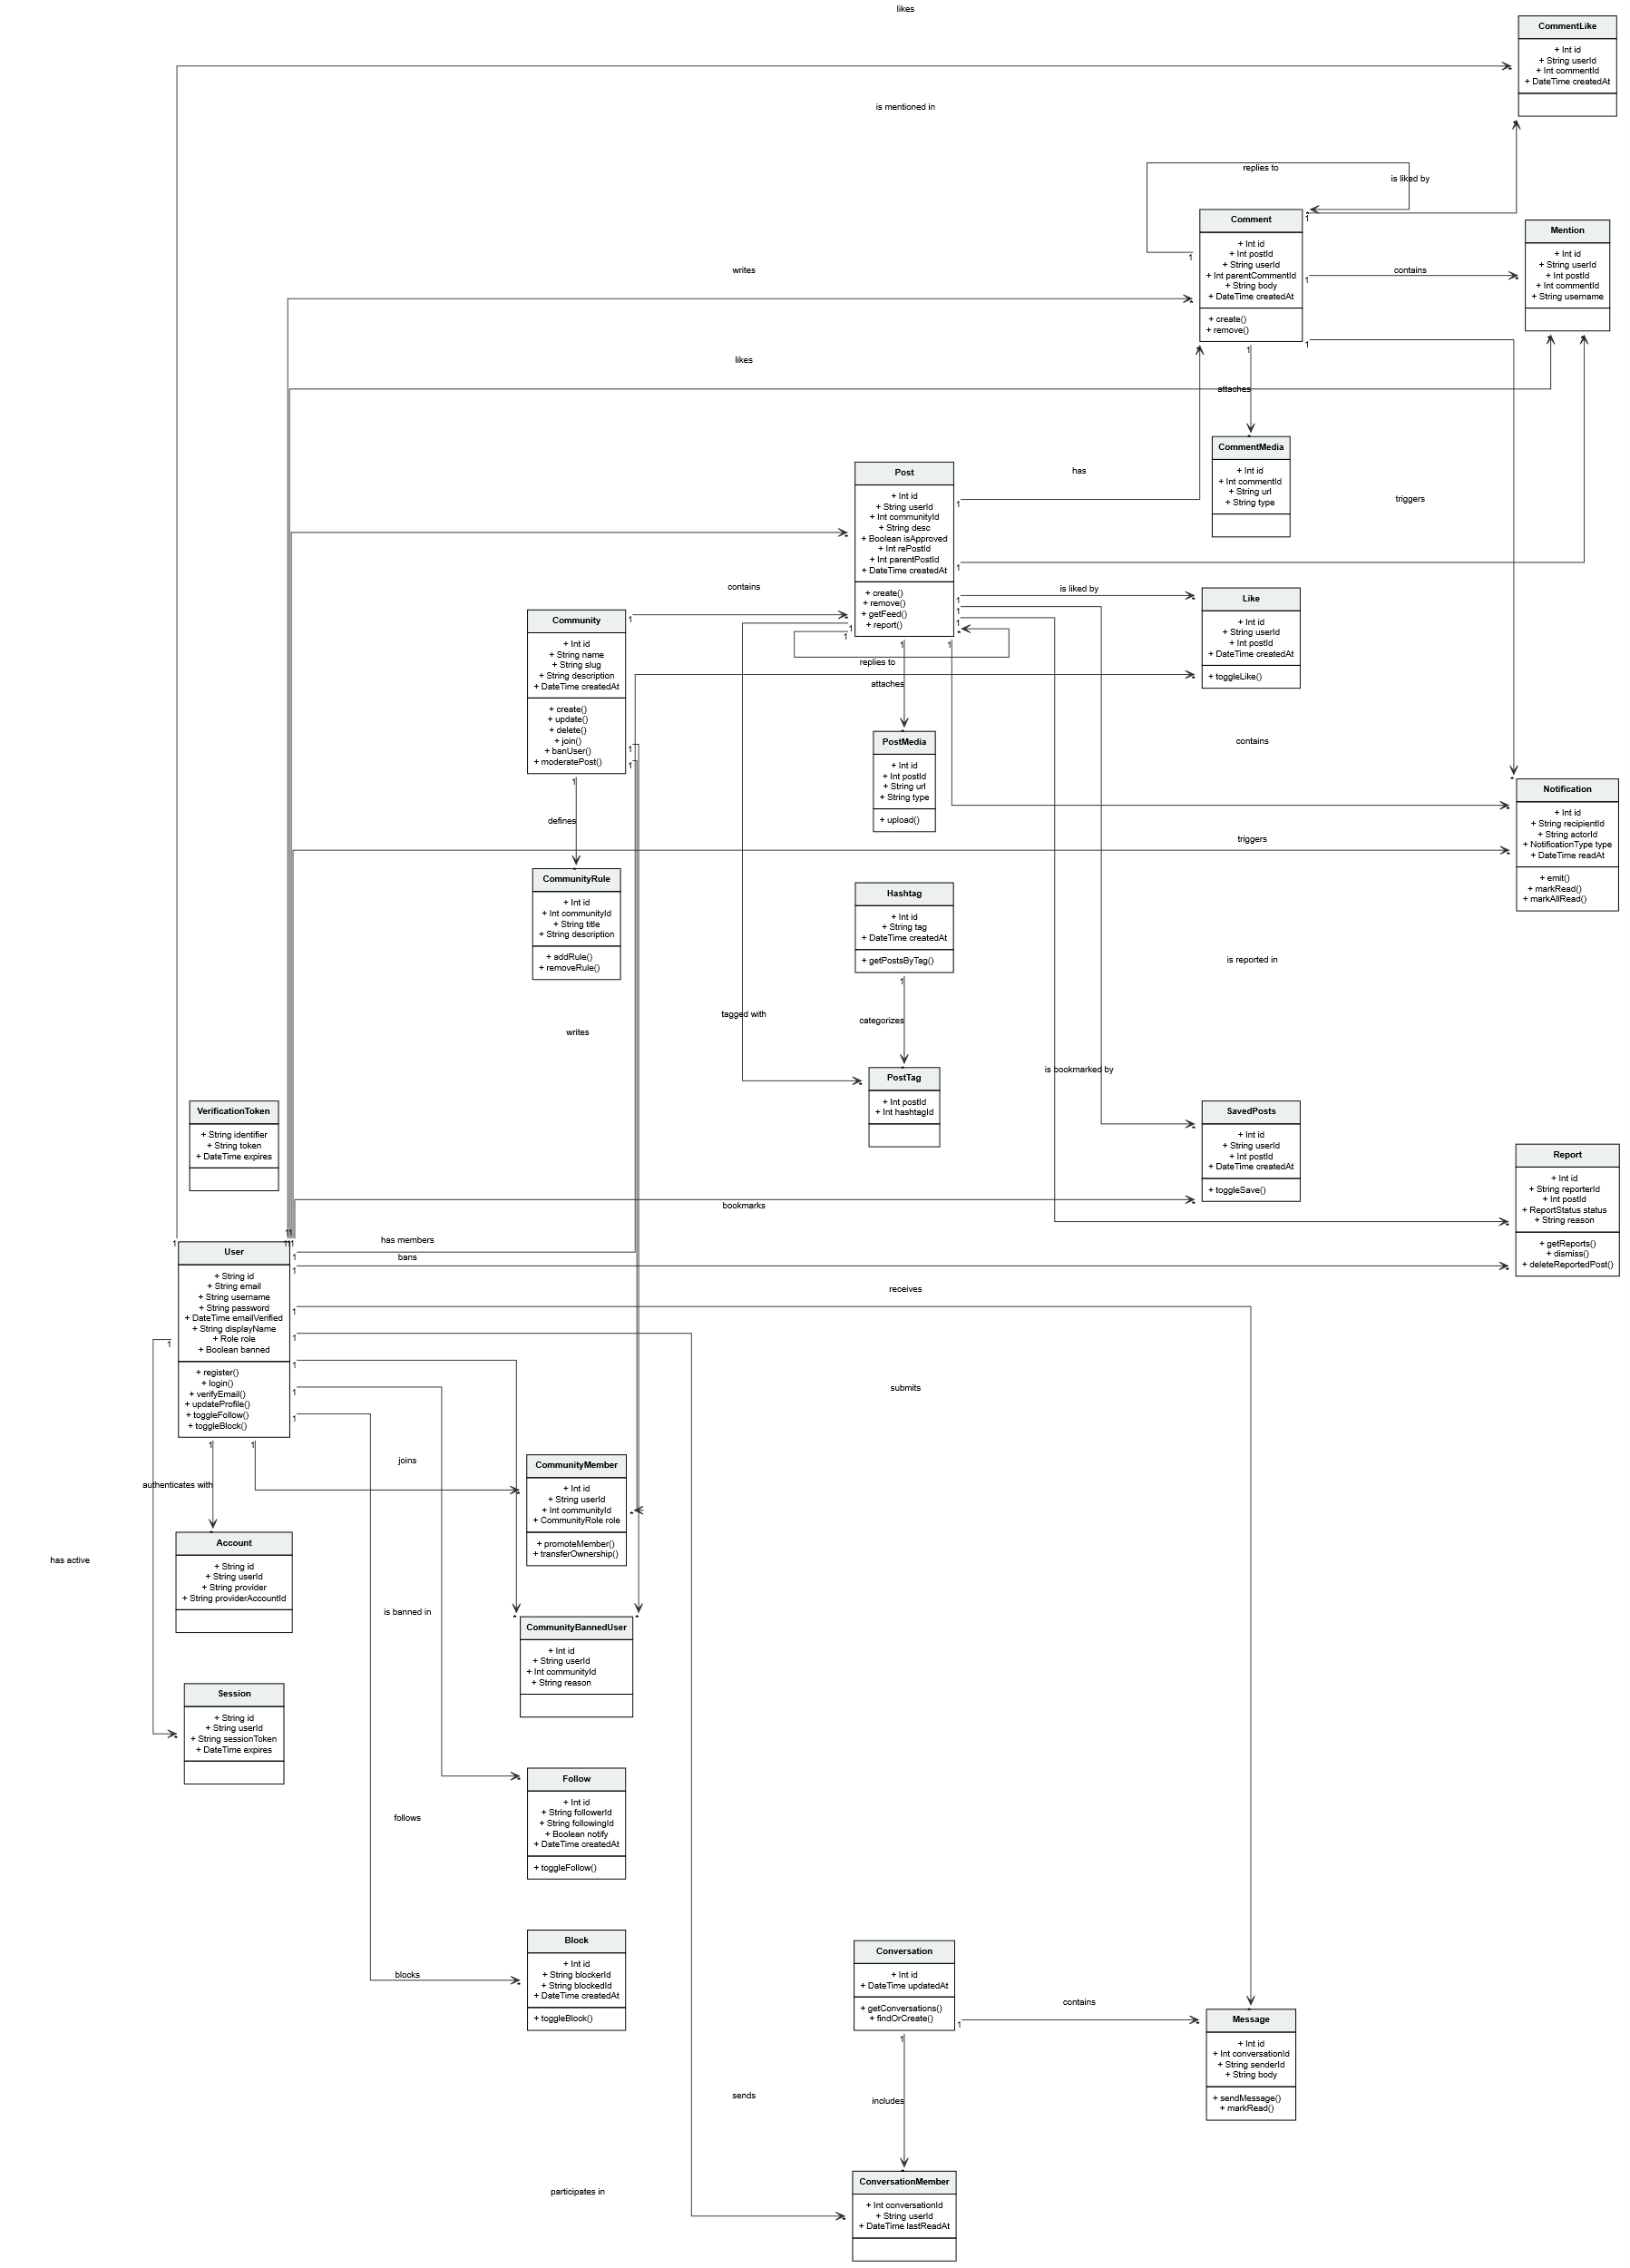
\includegraphics[width=0.92\linewidth,height=0.82\textheight,keepaspectratio]{images/image23.png}
  \caption{Class Diagram}
  \label{fig:19}
\end{figure}

Summary:
\begin{enumerate}
  \item Identity \& Access Domain Classes
\end{enumerate}

\begin{longtable}{|p{0.45\linewidth}|p{0.45\linewidth}|}
\caption{Identity \& Access Domain Classes} \label{tab:22} \\
\hline
\textbf{User}\newline Description: Core entity representing every platform account, storing identity and system-level access state.\newline Attributes:\newline id: String (PK)\newline email: String\newline username: String\newline password: String\newline emailVerified: DateTime\newline displayName: String\newline role: Role\newline banned: Boolean\newline Key Methods:\newline register(): Registers a new user\newline login(): Authenticates the user\newline verifyEmail(): Verifies email address\newline updateProfile(): Updates profile details\newline toggleFollow(): Follows or unfollows another user\newline toggleBlock(): Blocks or unblocks another user\newline Relationships:\newline Composition -> Account (one-to-many)\newline Composition -> Session (one-to-many)\newline Association -> Follow\newline Association -> Block\newline Association-> CommunityMember\newline Association -> Post\newline Association -> Comment\newline Association -> Notification & \textbf{VerificationToken}\newline Description: Stores single-use OTP codes for email verification and password reset.\newline Attributes:\newline identifier: String (PK)\newline token: String\newline expires: DateTime\newline Key Methods: None\newline Relationships: None \\
\hline
\endfirsthead
\multicolumn{2}{l}{\textit{(Continued from previous page)}} \\
\hline
\textbf{User}\newline Description: Core entity representing every platform account, storing identity and system-level access state.\newline Attributes:\newline id: String (PK)\newline email: String\newline username: String\newline password: String\newline emailVerified: DateTime\newline displayName: String\newline role: Role\newline banned: Boolean\newline Key Methods:\newline register(): Registers a new user\newline login(): Authenticates the user\newline verifyEmail(): Verifies email address\newline updateProfile(): Updates profile details\newline toggleFollow(): Follows or unfollows another user\newline toggleBlock(): Blocks or unblocks another user\newline Relationships:\newline Composition -> Account (one-to-many)\newline Composition -> Session (one-to-many)\newline Association -> Follow\newline Association -> Block\newline Association-> CommunityMember\newline Association -> Post\newline Association -> Comment\newline Association -> Notification & \textbf{VerificationToken}\newline Description: Stores single-use OTP codes for email verification and password reset.\newline Attributes:\newline identifier: String (PK)\newline token: String\newline expires: DateTime\newline Key Methods: None\newline Relationships: None \\
\hline
\endhead
\hline \multicolumn{2}{r}{\textit{Continued on next page}} \\
\endfoot
\hline
\endlastfoot
\end{longtable}

\begin{enumerate}
  \item Content Domain Classes
\end{enumerate}

\begin{longtable}{|p{0.45\linewidth}|p{0.45\linewidth}|}
\caption{Content Domain Classes} \label{tab:23} \\
\hline
\textbf{Post}\newline Description: Represents original posts, reposts, and quote-reposts.\newline Attributes:\newline id: Int (PK)\newline userId: String (FK)\newline communityId: Int (FK)\newline desc: String\newline isApproved: Boolean\newline rePostId: Int (FK)\newline parentPostId: Int (FK)\newline createdAt: DateTime\newline Key Methods:\newline create(): Creates a new post\newline remove(): Soft deletes the post\newline getFeed(): Retrieves post feed\newline report(): Reports the post\newline Relationships:\newline Association -> User\newline Association -> Community\newline Composition -> PostMedia (one-to-many)\newline Composition -> Comment (one-to-many)\newline Association -> PostTag (one-to-many) & \textbf{Comment}\newline Description: User replies to a Post, supporting nested comment threads.\newline Attributes:\newline id: Int (PK)\newline postId: Int (FK)\newline userId: String (FK)\newline parentCommentId: Int (FK)\newline body: String\newline createdAt: DateTime\newline Key Methods:\newline create(): Adds a comment\newline remove(): Removes a comment\newline Relationships:\newline Association -> User\newline Association -> Post\newline Composition -> CommentMedia (one-to-many) \\
\hline
\endfirsthead
\multicolumn{2}{l}{\textit{(Continued from previous page)}} \\
\hline
\textbf{Post}\newline Description: Represents original posts, reposts, and quote-reposts.\newline Attributes:\newline id: Int (PK)\newline userId: String (FK)\newline communityId: Int (FK)\newline desc: String\newline isApproved: Boolean\newline rePostId: Int (FK)\newline parentPostId: Int (FK)\newline createdAt: DateTime\newline Key Methods:\newline create(): Creates a new post\newline remove(): Soft deletes the post\newline getFeed(): Retrieves post feed\newline report(): Reports the post\newline Relationships:\newline Association -> User\newline Association -> Community\newline Composition -> PostMedia (one-to-many)\newline Composition -> Comment (one-to-many)\newline Association -> PostTag (one-to-many) & \textbf{Comment}\newline Description: User replies to a Post, supporting nested comment threads.\newline Attributes:\newline id: Int (PK)\newline postId: Int (FK)\newline userId: String (FK)\newline parentCommentId: Int (FK)\newline body: String\newline createdAt: DateTime\newline Key Methods:\newline create(): Adds a comment\newline remove(): Removes a comment\newline Relationships:\newline Association -> User\newline Association -> Post\newline Composition -> CommentMedia (one-to-many) \\
\hline
\endhead
\hline \multicolumn{2}{r}{\textit{Continued on next page}} \\
\endfoot
\hline
\endlastfoot
PostMedia\newline Description: Stores image and video attachments for a Post.\newline Attributes:\newline id: Int (PK)\newline postId: Int (FK)\newline url: String\newline type: String\newline Key Methods:\newline upload(): Uploads media file\newline Relationships:\newline Association -> Post & CommentMedia\newline Description: File attachments embedded inside comments.\newline Attributes:\newline id: Int (PK)\newline commentId: Int (FK)\newline url: String\newline type: String\newline Relationships:\newline Association -> Comment \\
\hline
Hashtag \& PostTag\newline Description: Registry of tags and the junction class link Posts to Hashtags.\newline Key Methods:\newline getPostsByTag(): Retrieves posts by hashtag\newline Relationships:\newline Association -> Post &  \\
\hline
\end{longtable}

\begin{enumerate}
  \item Social Engagement Domain Classes
\end{enumerate}

\begin{longtable}{|p{0.45\linewidth}|p{0.45\linewidth}|}
\caption{Social Engagement Domain Classes} \label{tab:24} \\
\hline
\textbf{Follow}\newline Description: Directed social graph edge for user following.\newline Attributes:\newline id: Int (PK)\newline followerId: String (FK)\newline followingId: String (FK)\newline notify: Boolean\newline createdAt: DateTime\newline Key Methods:\newline toggleFollow(): Follows/unfollows\newline Relationships:\newline Association -> User & \textbf{Like}\newline Description: Records a User's reaction on a Post.\newline Attributes:\newline id: Int (PK)\newline userId: String (FK)\newline postId: Int (FK)\newline createdAt: DateTime\newline Key Methods:\newline toggleLike(): Likes/ unlikes a post\newline Relationships:\newline Association -> User\newline Association -> Post \\
\hline
\endfirsthead
\multicolumn{2}{l}{\textit{(Continued from previous page)}} \\
\hline
\textbf{Follow}\newline Description: Directed social graph edge for user following.\newline Attributes:\newline id: Int (PK)\newline followerId: String (FK)\newline followingId: String (FK)\newline notify: Boolean\newline createdAt: DateTime\newline Key Methods:\newline toggleFollow(): Follows/unfollows\newline Relationships:\newline Association -> User & \textbf{Like}\newline Description: Records a User's reaction on a Post.\newline Attributes:\newline id: Int (PK)\newline userId: String (FK)\newline postId: Int (FK)\newline createdAt: DateTime\newline Key Methods:\newline toggleLike(): Likes/ unlikes a post\newline Relationships:\newline Association -> User\newline Association -> Post \\
\hline
\endhead
\hline \multicolumn{2}{r}{\textit{Continued on next page}} \\
\endfoot
\hline
\endlastfoot
Block\newline Description: Mutual blacklist between two users.\newline Attributes:\newline id: Int (PK)\newline blockerId: String (FK)\newline blockedId: String (FK)\newline createdAt: DateTime\newline Key Methods:\newline toggleBlock(): Blocks or unblocks a user\newline Relationships:\newline Association -> User & SavedPost\newline Description: User's personal bookmark list.\newline Attributes:\newline id: Int (PK)\newline userId: String (FK)\newline postId: Int (FK)\newline createdAt: DateTime\newline Key Methods:\newline toggleSave(): Save/unsave a post\newline Relationships:\newline Association -> User\newline Association -> Post \\
\hline
Mention\newline Description: Records @username tags inside content.\newline Attributes:\newline id: Int (PK)\newline userId: String (FK)\newline postId: Int (FK)\newline commentId: Int (FK)\newline username: String\newline Relationships:\newline Association -> User, Post, Comment & CommentLike\newline Description: Records a User's reaction on a Comment.\newline Attributes:\newline id: Int (PK)\newline userId: String (FK)\newline commentID: Int (FK)\newline Relationships:\newline Association -> User\newline Association -> Comment \\
\hline
\end{longtable}

\begin{enumerate}
  \item Community \& Moderation Domain Classes
\end{enumerate}

\begin{longtable}{|p{0.45\linewidth}|p{0.45\linewidth}|}
\caption{Community \& Moderation Domain Classes} \label{tab:25} \\
\hline
\textbf{Community}\newline Description: A shared space for members with a common interest.\newline Attributes:\newline id: Int (PK)\newline name: String\newline slug: String\newline description: String\newline createdAt: DateTime\newline Key Methods:\newline create(): Creates a new community\newline update(): Update community detail\newline delete(): Deletes the community\newline join(): Joins/ leaves the community\newline banUser(): Bans a user from the community\newline moderatePost(): Approves/rejects a post\newline Relationships:\newline Composition -> CommunityMember\newline Composition -> CommunityRule\newline Composition-> CommunityBannedUser\newline Composition -> Post & \textbf{CommunityMember}\newline Description: Manages community members and their roles.\newline Attributes:\newline id: Int (PK)\newline userId: String (FK)\newline communityId: Int (FK)\newline role: CommunityRole\newline Key Methods:\newline promoteMember(): Promotes a member to moderator\newline transferOwnership(): Transfers community ownership\newline Relationships:\newline Association -> Community\newline Association -> User \\
\hline
\endfirsthead
\multicolumn{2}{l}{\textit{(Continued from previous page)}} \\
\hline
\textbf{Community}\newline Description: A shared space for members with a common interest.\newline Attributes:\newline id: Int (PK)\newline name: String\newline slug: String\newline description: String\newline createdAt: DateTime\newline Key Methods:\newline create(): Creates a new community\newline update(): Update community detail\newline delete(): Deletes the community\newline join(): Joins/ leaves the community\newline banUser(): Bans a user from the community\newline moderatePost(): Approves/rejects a post\newline Relationships:\newline Composition -> CommunityMember\newline Composition -> CommunityRule\newline Composition-> CommunityBannedUser\newline Composition -> Post & \textbf{CommunityMember}\newline Description: Manages community members and their roles.\newline Attributes:\newline id: Int (PK)\newline userId: String (FK)\newline communityId: Int (FK)\newline role: CommunityRole\newline Key Methods:\newline promoteMember(): Promotes a member to moderator\newline transferOwnership(): Transfers community ownership\newline Relationships:\newline Association -> Community\newline Association -> User \\
\hline
\endhead
\hline \multicolumn{2}{r}{\textit{Continued on next page}} \\
\endfoot
\hline
\endlastfoot
CommunityBannedUser\newline Description: Community-level blacklist enforced by Moderators.\newline Attributes:\newline id: Int (PK)\newline userId: String (FK)\newline communityId: Int (FK)\newline reason: String\newline Relationships:\newline Association -> User\newline Association -> Community & CommunityRule\newline Description: Custom rules set by the community.\newline Attributes:\newline id: Int (PK)\newline communityId: Int (FK)\newline title: String\newline description: String\newline Key Methods:\newline addRule(): Adds a new rule\newline removeRule(): Removes a rule\newline Relationships\newline Association -> Community \\
\hline
\end{longtable}

\begin{enumerate}
  \item Communication Domain Classes
\end{enumerate}

\begin{longtable}{|p{0.45\linewidth}|p{0.45\linewidth}|}
\caption{Communication Domain Classes} \label{tab:26} \\
\hline
\textbf{ShopOrder}\newline Description: Represents a direct message thread.\newline Attributes:\newline id: Int (PK)\newline updateAt: DateTime\newline Key Methods:\newline getConversations(): Retrieves user conversations\newline findOrCreate(): Finds or creates a conversation thread\newline Relationships:\newline Composition -> ConversationMember (one-to-many)\newline Composition -> Message (one-to-many) & \textbf{Notification}\newline Description: System-generated alert\newline Attributes:\newline id: Int (PK)\newline recipientId: String (FK)\newline actorId: String (FK)\newline type: NotificationType\newline readAt: DateTime\newline Key Methods:\newline emit(): Emits real-time notification\newline markRead(): Marks notification\newline markAllRead(): Marks all notifications as read\newline Relationships:\newline Association -> User\newline Association -> Post\newline Association -> Comment \\
\hline
\endfirsthead
\multicolumn{2}{l}{\textit{(Continued from previous page)}} \\
\hline
\textbf{ShopOrder}\newline Description: Represents a direct message thread.\newline Attributes:\newline id: Int (PK)\newline updateAt: DateTime\newline Key Methods:\newline getConversations(): Retrieves user conversations\newline findOrCreate(): Finds or creates a conversation thread\newline Relationships:\newline Composition -> ConversationMember (one-to-many)\newline Composition -> Message (one-to-many) & \textbf{Notification}\newline Description: System-generated alert\newline Attributes:\newline id: Int (PK)\newline recipientId: String (FK)\newline actorId: String (FK)\newline type: NotificationType\newline readAt: DateTime\newline Key Methods:\newline emit(): Emits real-time notification\newline markRead(): Marks notification\newline markAllRead(): Marks all notifications as read\newline Relationships:\newline Association -> User\newline Association -> Post\newline Association -> Comment \\
\hline
\endhead
\hline \multicolumn{2}{r}{\textit{Continued on next page}} \\
\endfoot
\hline
\endlastfoot
ConservationMember\newline Description: Junction class tracking conversation participants.\newline Attributes:\newline conversationId: Int (FK)\newline userId: String (FK)\newline lastReadAt: DateTime\newline Relationships:\newline Association -> User\newline Association -> Conversation & Report\newline Description: Content flagging system for moderation.\newline Attributes:\newline id: Int (PK)\newline reporterId: String (FK)\newline postId: Int (FK)\newline status: ReportStatus\newline reason: String\newline Key Methods:\newline getReports(): Retrieves list post\newline dismiss(): Dismisses a report\newline deleteReportedPost(): Deletes the reported post\newline Relationships:\newline Association -> User\newline Association -> Post \\
\hline
Message\newline Description: Individual message within a conversation.\newline Attributes:\newline id: Int (PK)\newline conversationId: Int (FK)\newline senderId: String (FK)\newline body: String\newline Key Methods:\newline sendMessage(): Sends a new message\newline markRead(): Marks message as read\newline Relationships:\newline Association -> User\newline Association -> Conservation &  \\
\hline
\end{longtable}


\subsubsection{Sequence Diagram}

This section presents ten sequence diagrams that model the dynamic behavior of the Breadit social network, mapping directly to its core use cases. These diagrams visualize the runtime interactions between the user, Next.js frontend, NestJS backend API, PostgreSQL database (via Prisma), and real-time Socket.IO/Redis pipeline. The illustrated flows cover: (1) Authentication, (2) Content Discovery, (3) Post Management, (4) Post Interaction, (5) Relationship Management, (6) Profile Management, (7) Direct Messaging, (8) Real-Time Notifications, (9) Community Management, and (10) Administrative Moderation.

\medskip\noindent\textbf{Authentication \& Account Management}\\[2pt]
\begin{figure}[H]
  \centering
  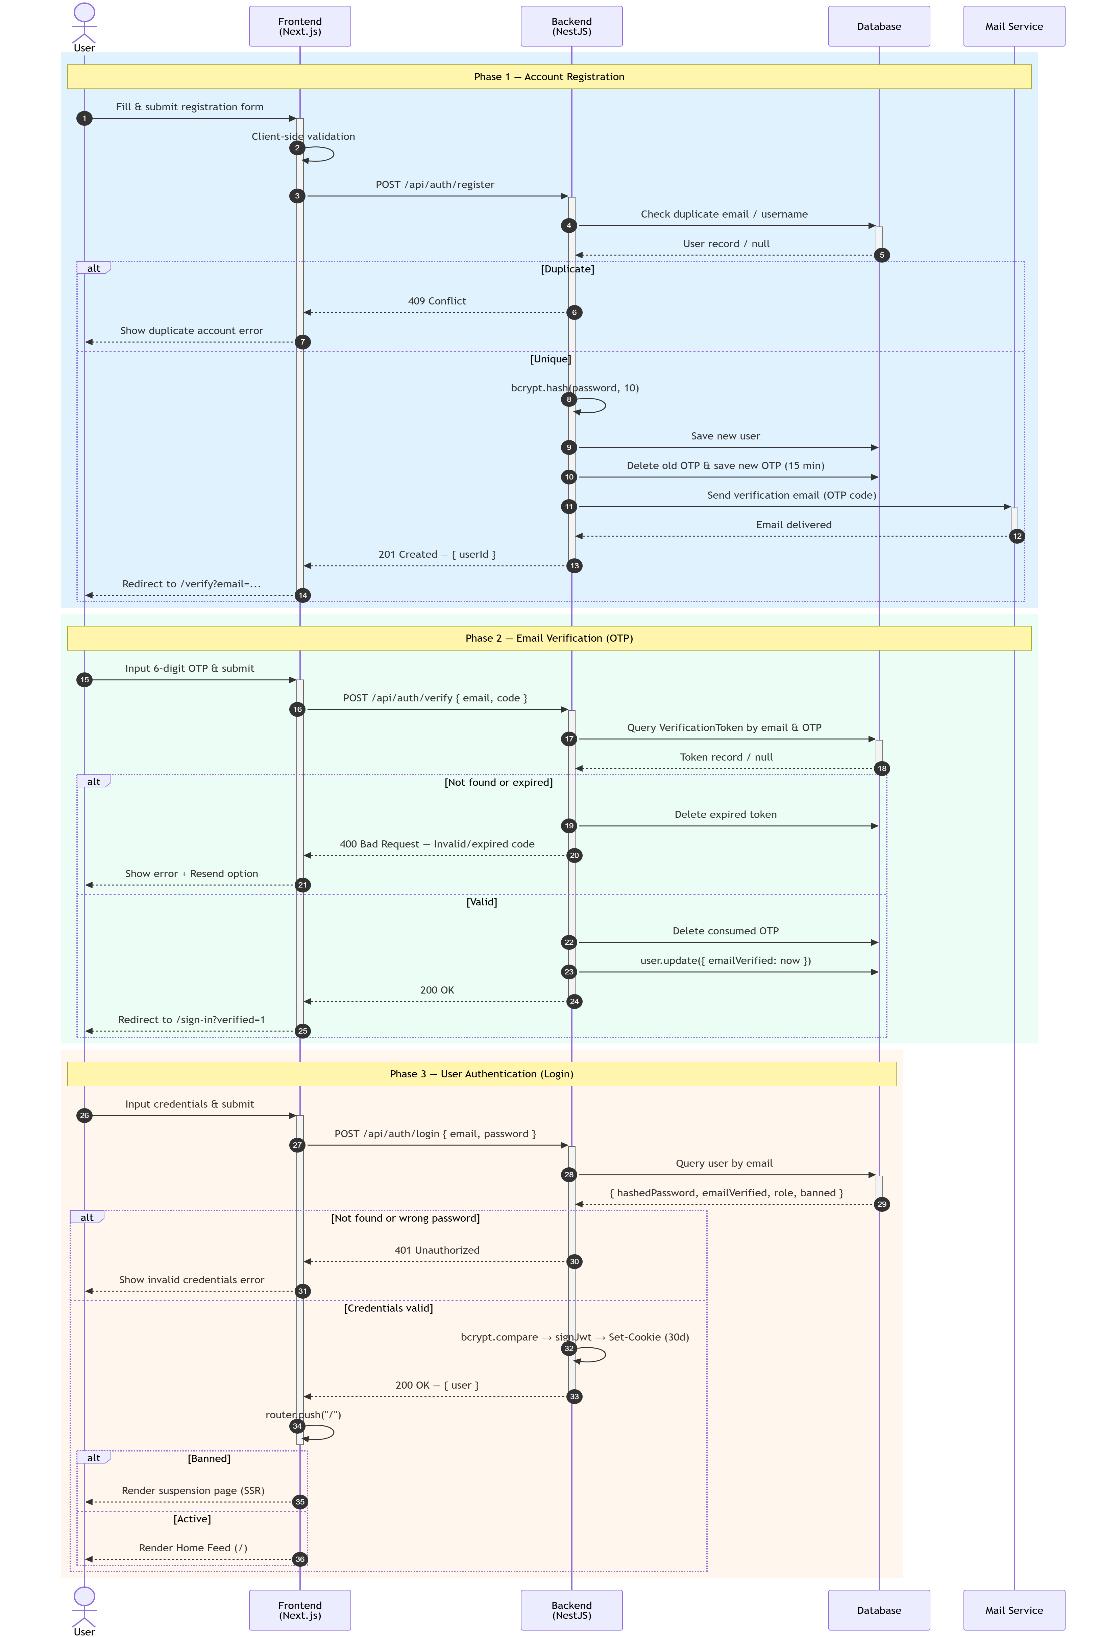
\includegraphics[width=0.92\linewidth,height=0.82\textheight,keepaspectratio]{images/image25.png}
  \caption{Authentication \& Account Management Diagram}
  \label{fig:20}
\end{figure}

\medskip\noindent\textbf{Feeds and Discovery}\\[2pt]
\begin{figure}[H]
  \centering
  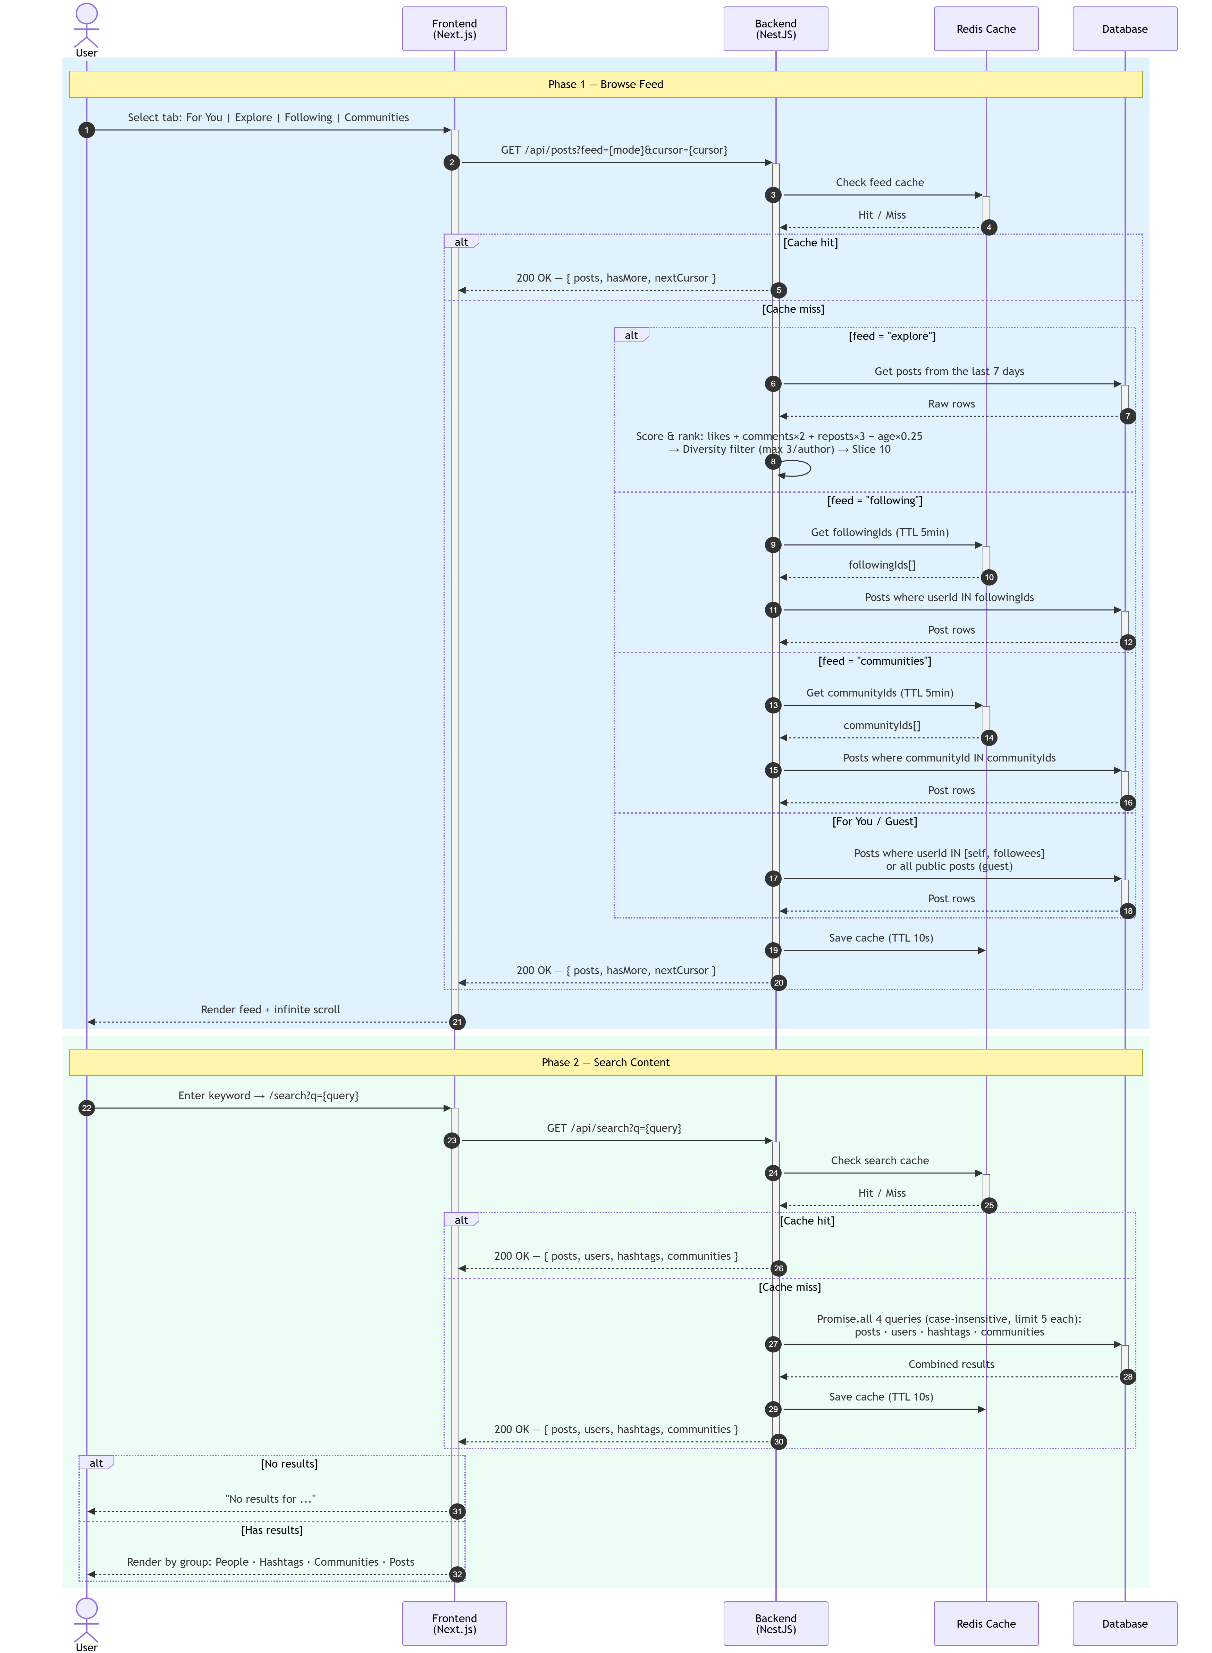
\includegraphics[width=0.92\linewidth,height=0.82\textheight,keepaspectratio]{images/image26.png}
  \caption{Feeds and Discovery Diagram}
  \label{fig:21}
\end{figure}

\medskip\noindent\textbf{Post Management}\\[2pt]
\begin{figure}[H]
  \centering
  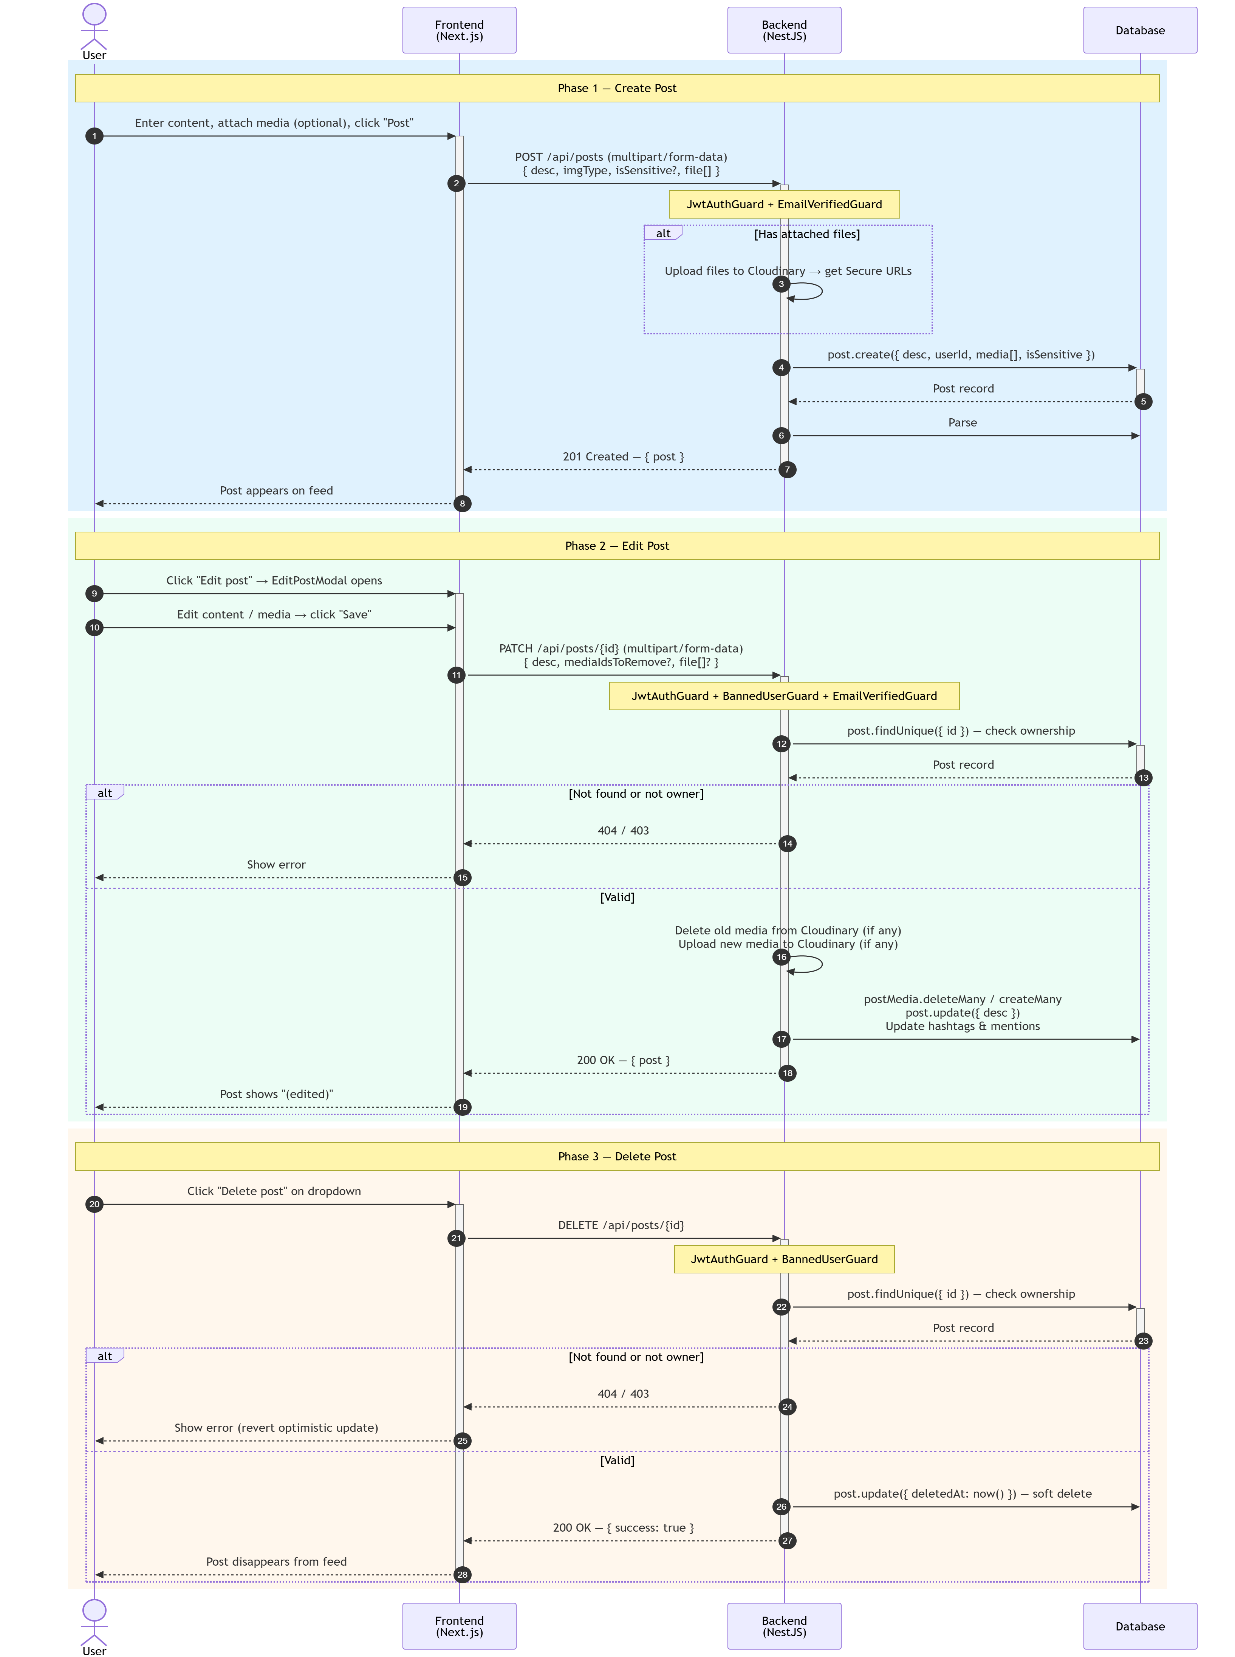
\includegraphics[width=0.92\linewidth,height=0.82\textheight,keepaspectratio]{images/image27.png}
  \caption{Post Management Diagram}
  \label{fig:22}
\end{figure}

\medskip\noindent\textbf{Post Interaction}\\[2pt]
\begin{figure}[H]
  \centering
  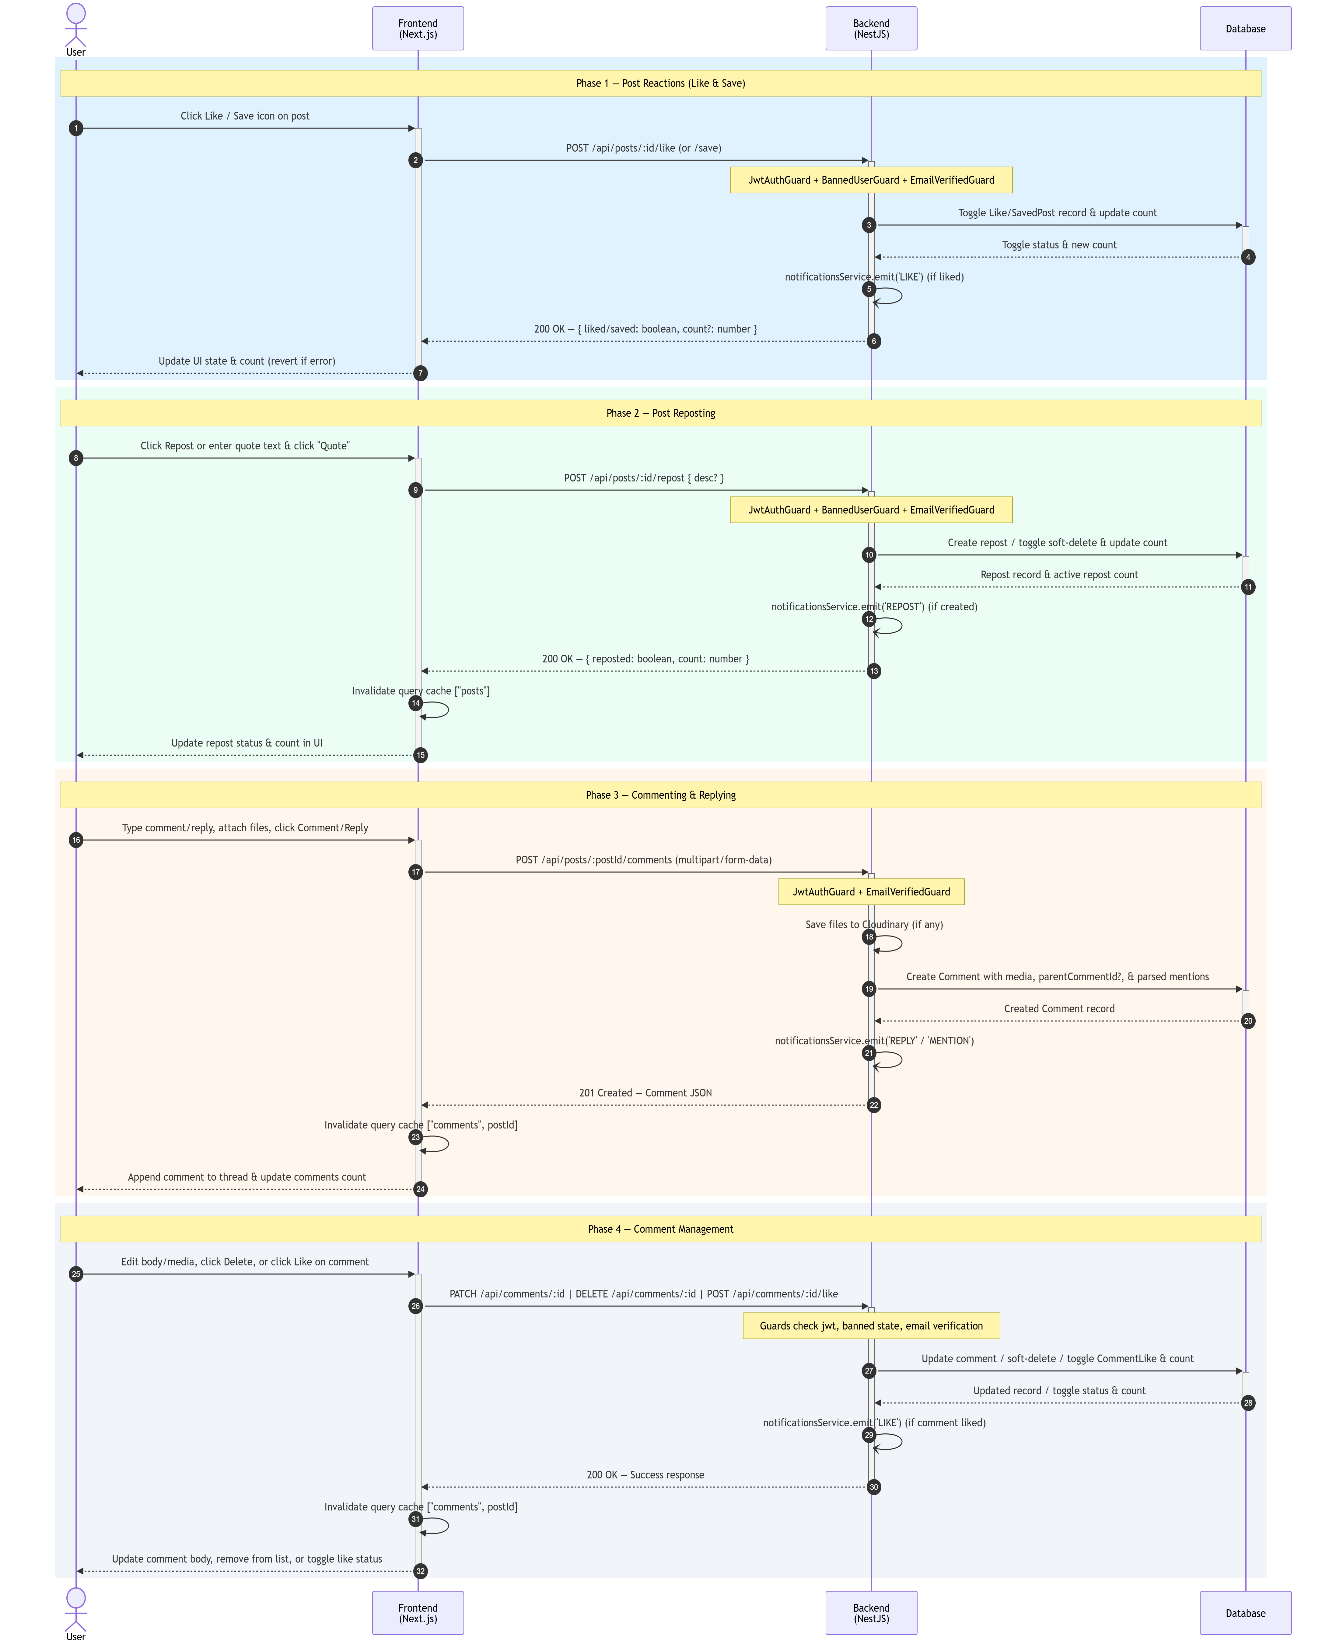
\includegraphics[width=0.92\linewidth,height=0.82\textheight,keepaspectratio]{images/image28.png}
  \caption{Post Interaction Diagram}
  \label{fig:23}
\end{figure}

\medskip\noindent\textbf{User Relationship Management}\\[2pt]
\begin{figure}[H]
  \centering
  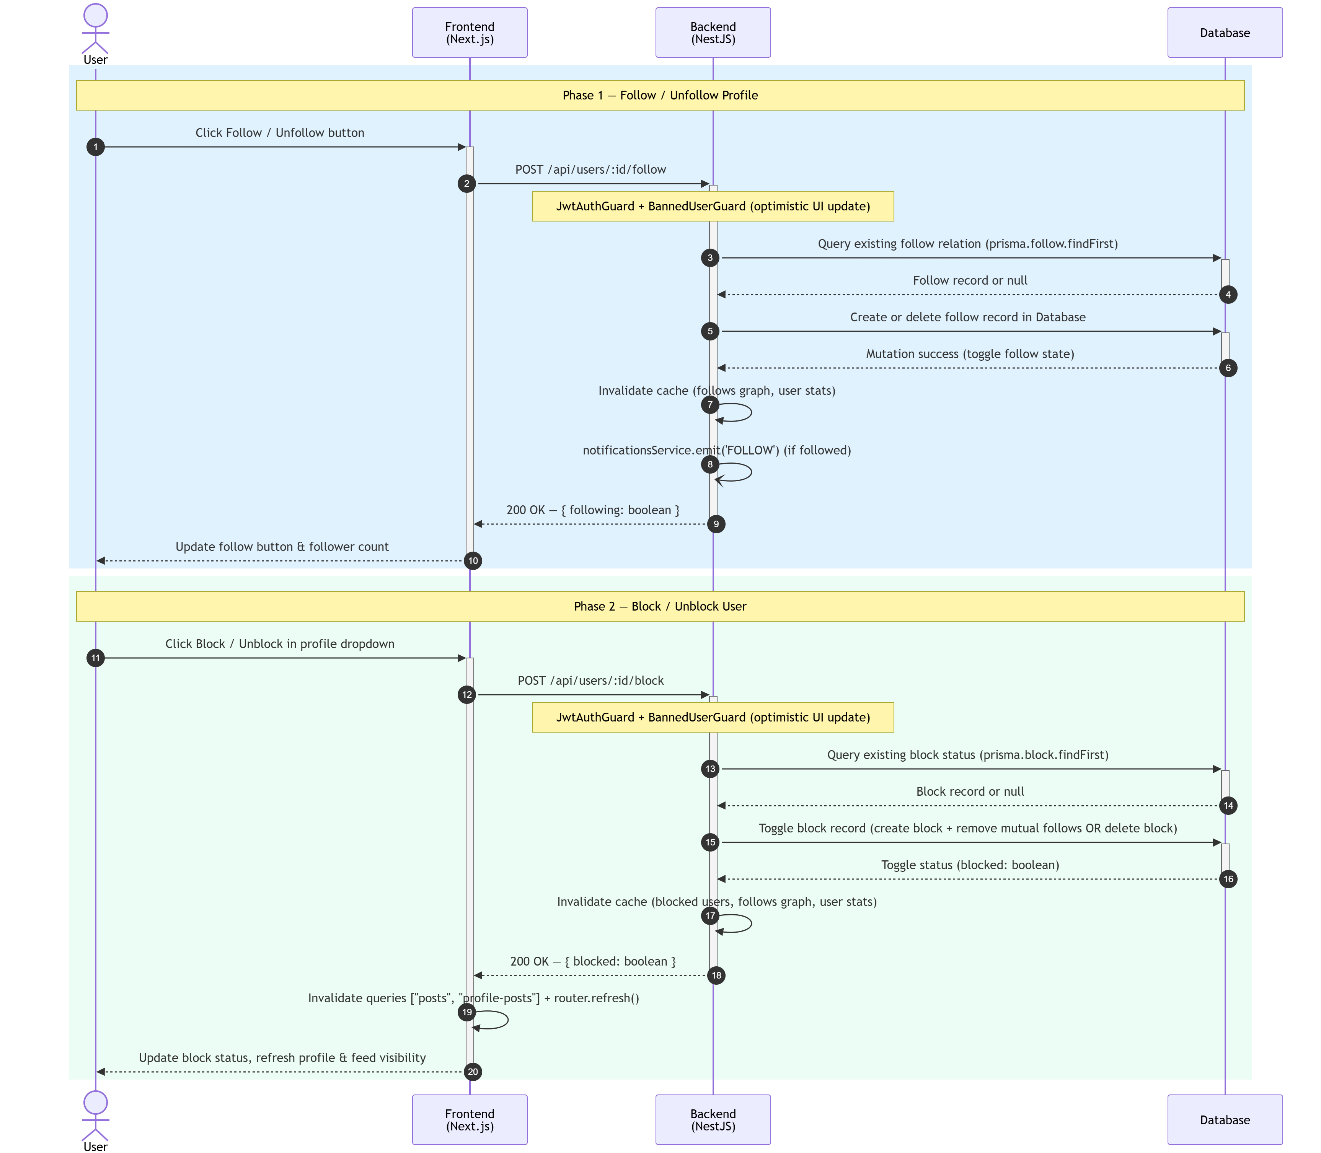
\includegraphics[width=0.92\linewidth,height=0.82\textheight,keepaspectratio]{images/image29.png}
  \caption{User Relationship Management Diagram}
  \label{fig:24}
\end{figure}

\medskip\noindent\textbf{User Profile Management}\\[2pt]
\begin{figure}[H]
  \centering
  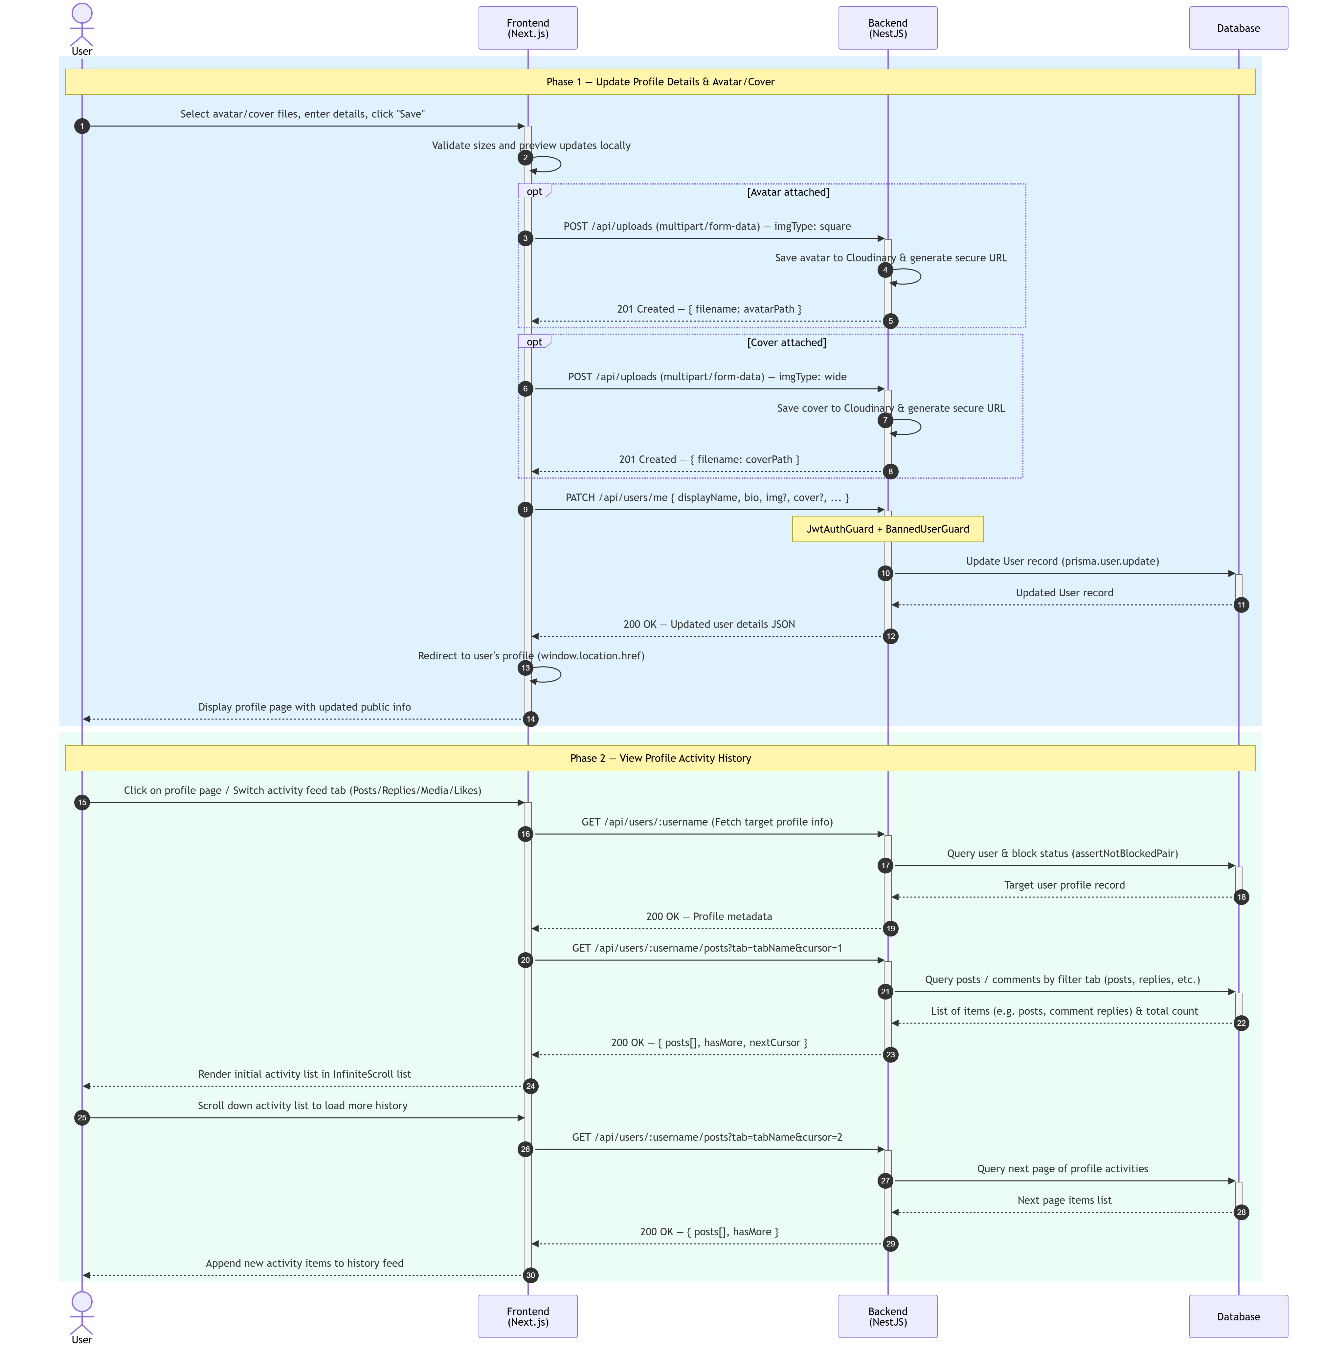
\includegraphics[width=0.92\linewidth,height=0.82\textheight,keepaspectratio]{images/image30.png}
  \caption{User Profile Management Diagram}
  \label{fig:25}
\end{figure}

\medskip\noindent\textbf{Direct Messaging}\\[2pt]
\begin{figure}[H]
  \centering
  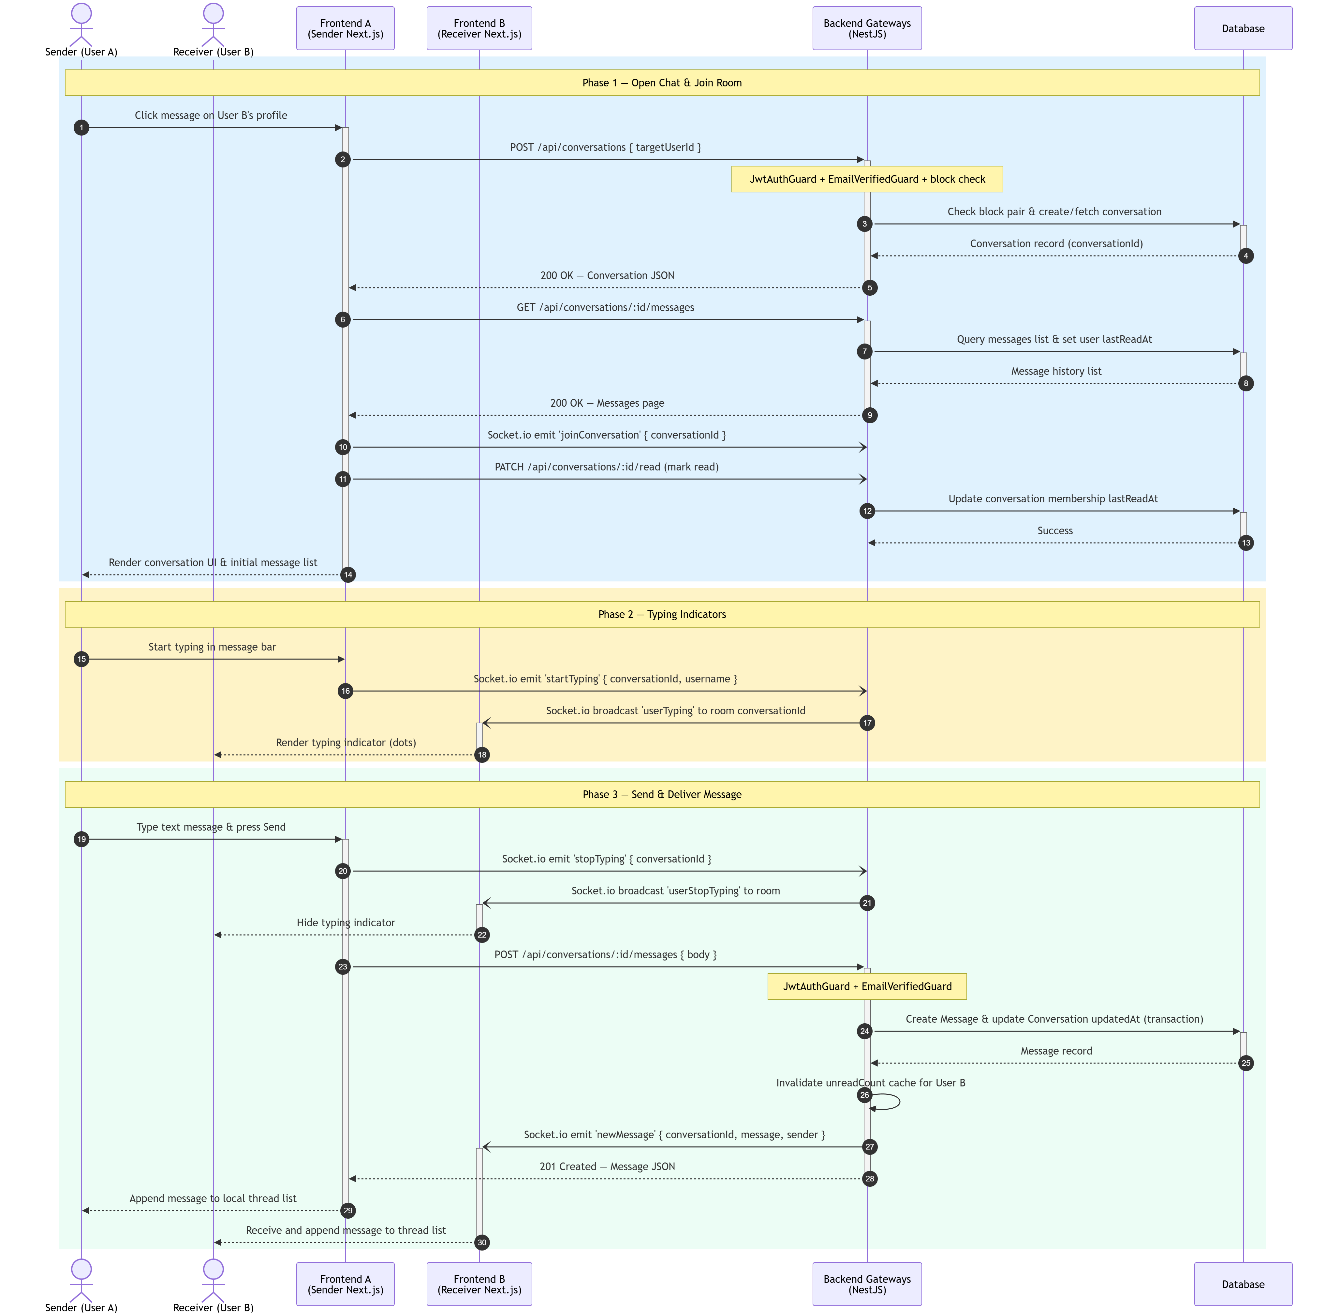
\includegraphics[width=0.92\linewidth,height=0.82\textheight,keepaspectratio]{images/image31.png}
  \caption{Direct Messaging Diagram}
  \label{fig:26}
\end{figure}

\medskip\noindent\textbf{Real-time Notifications}\\[2pt]
\begin{figure}[H]
  \centering
  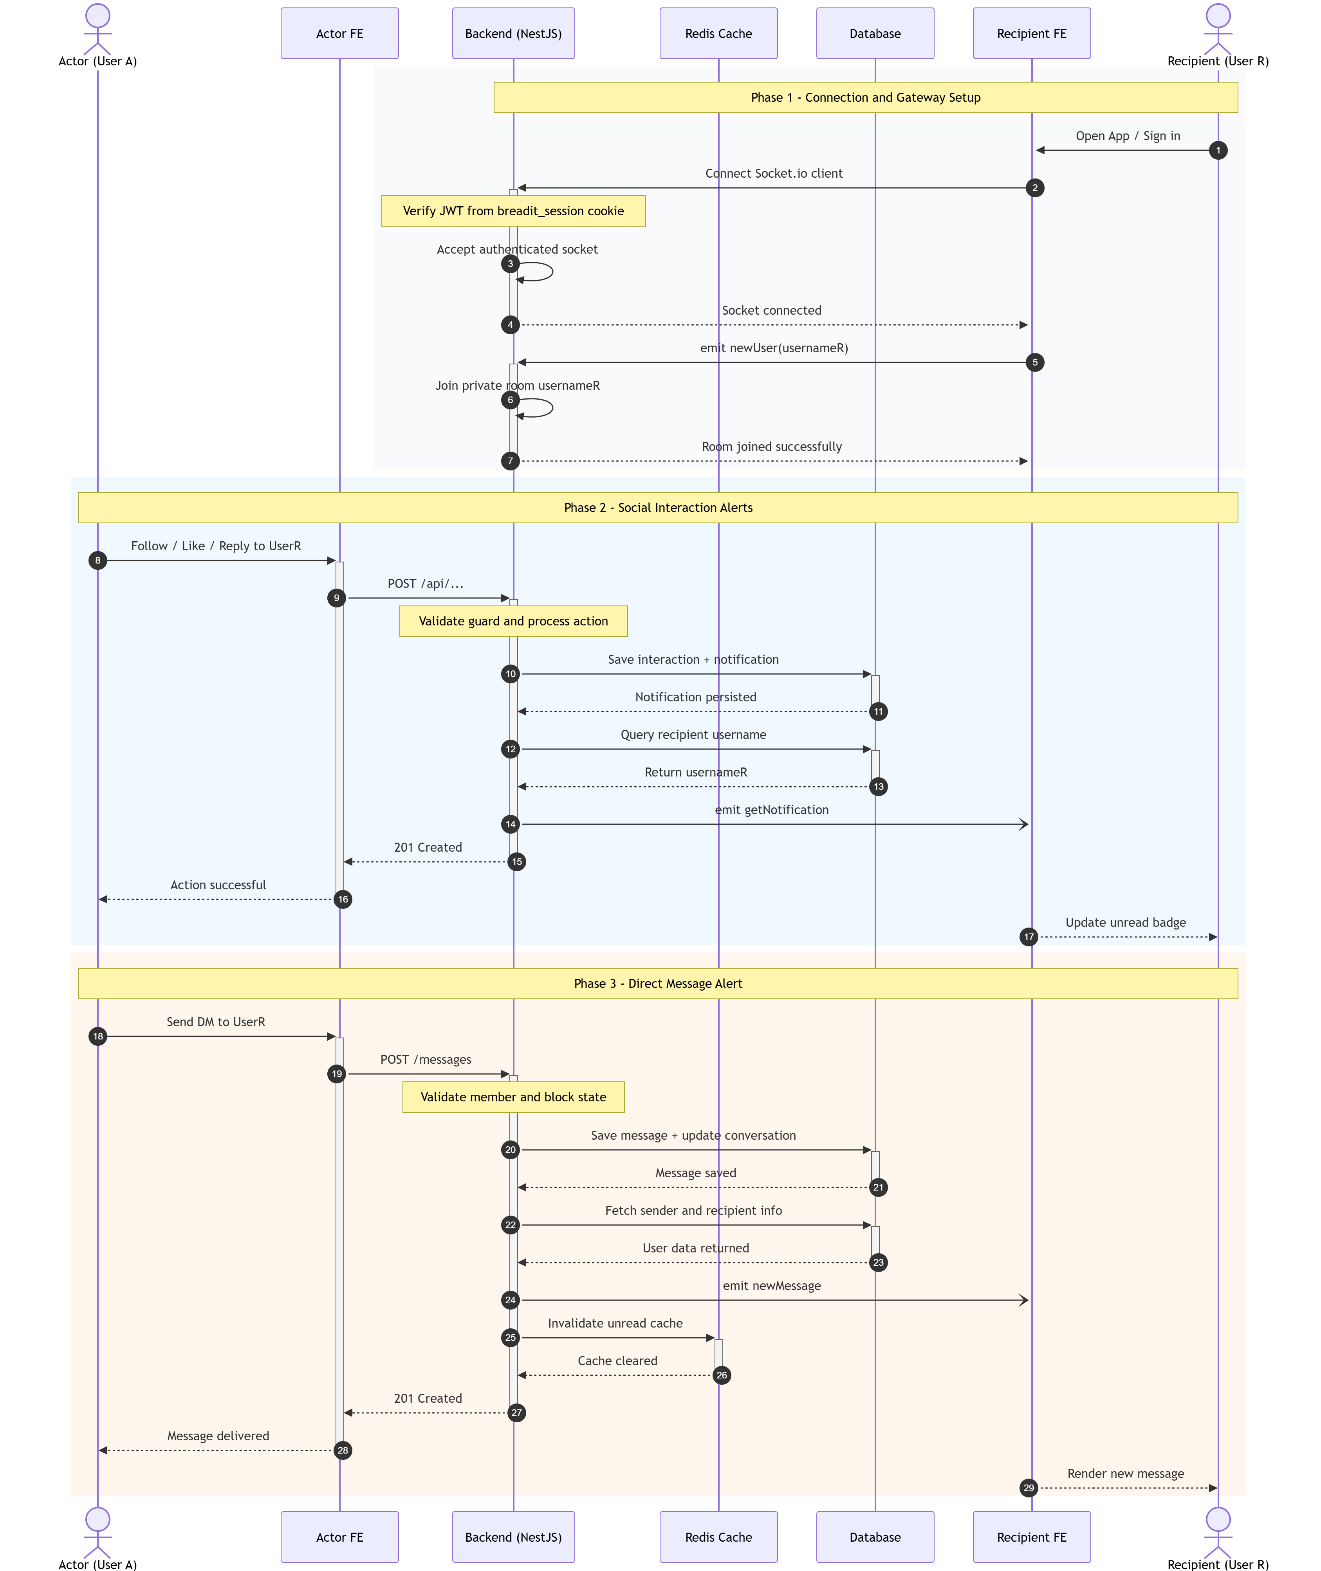
\includegraphics[width=0.92\linewidth,height=0.82\textheight,keepaspectratio]{images/image32.png}
  \caption{Real-time Notifications Diagram}
  \label{fig:27}
\end{figure}

\medskip\noindent\textbf{Community Management}\\[2pt]
\begin{figure}[H]
  \centering
  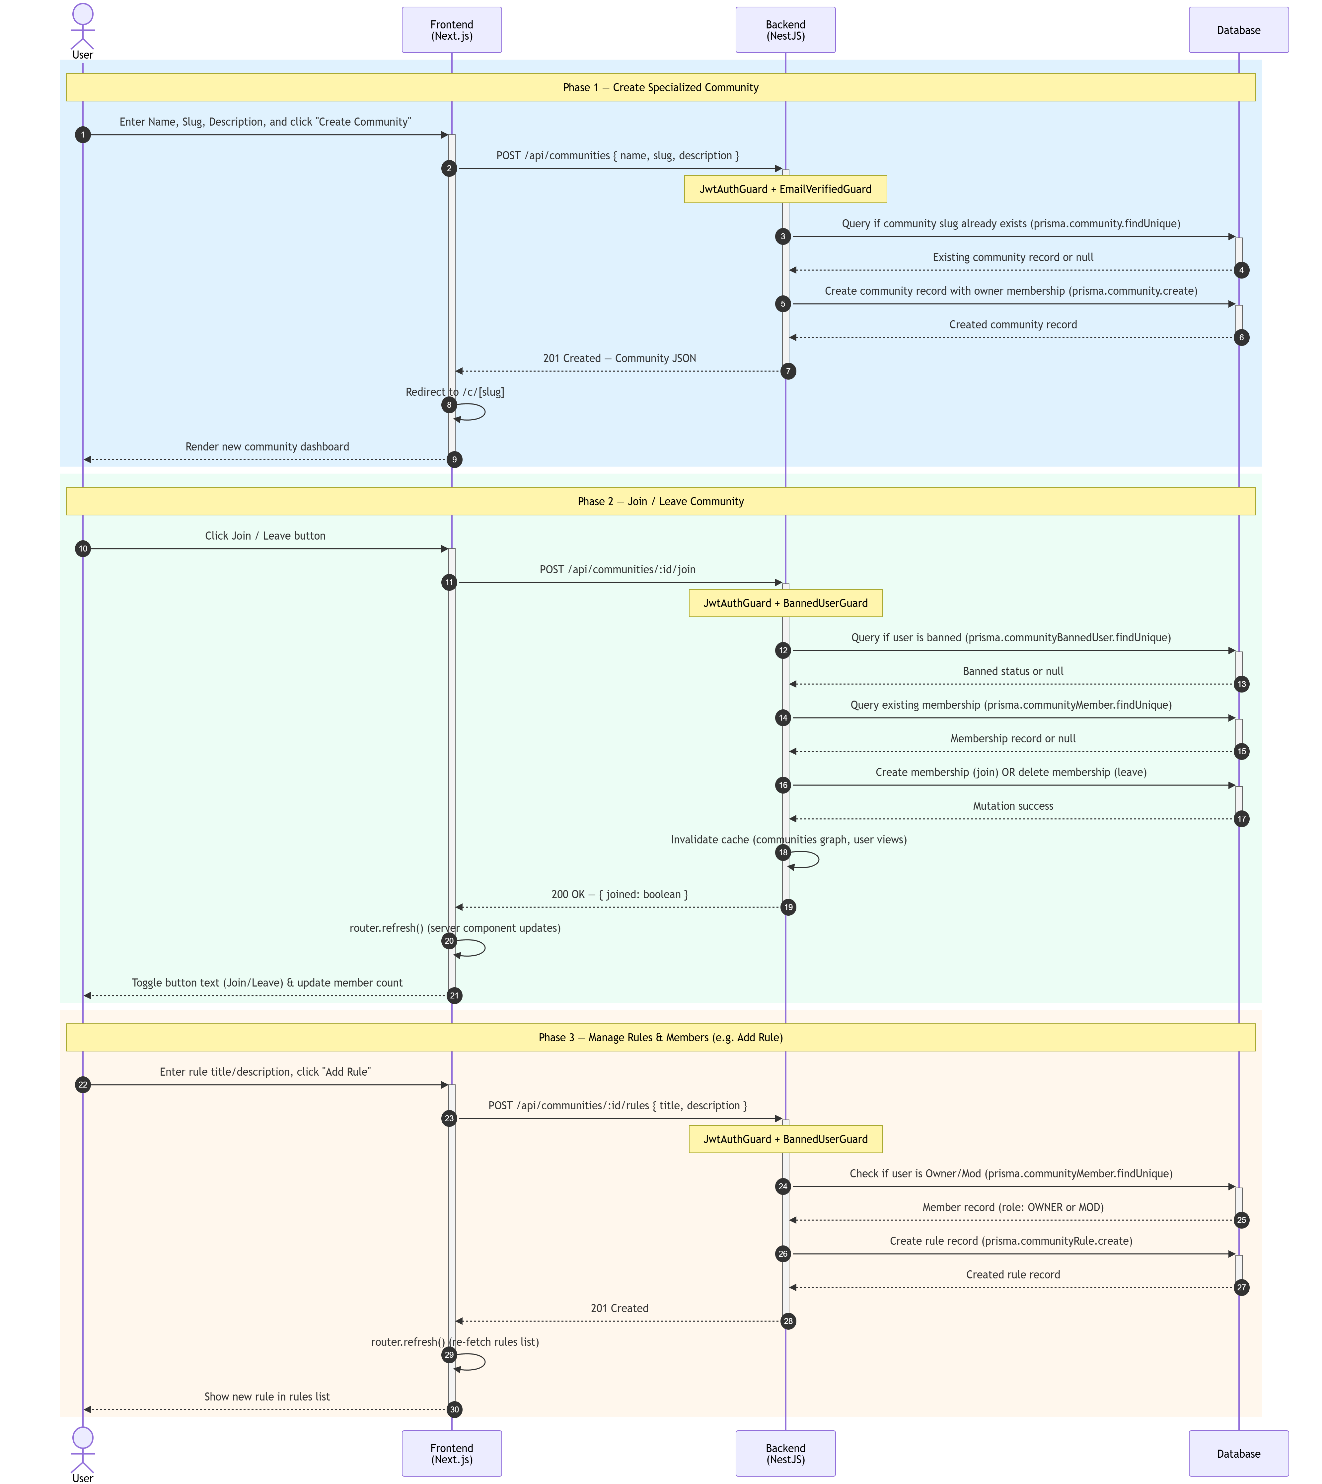
\includegraphics[width=0.92\linewidth,height=0.82\textheight,keepaspectratio]{images/image33.png}
  \caption{Community Management Diagram}
  \label{fig:28}
\end{figure}

\medskip\noindent\textbf{Administrative Moderation}\\[2pt]
\begin{figure}[H]
  \centering
  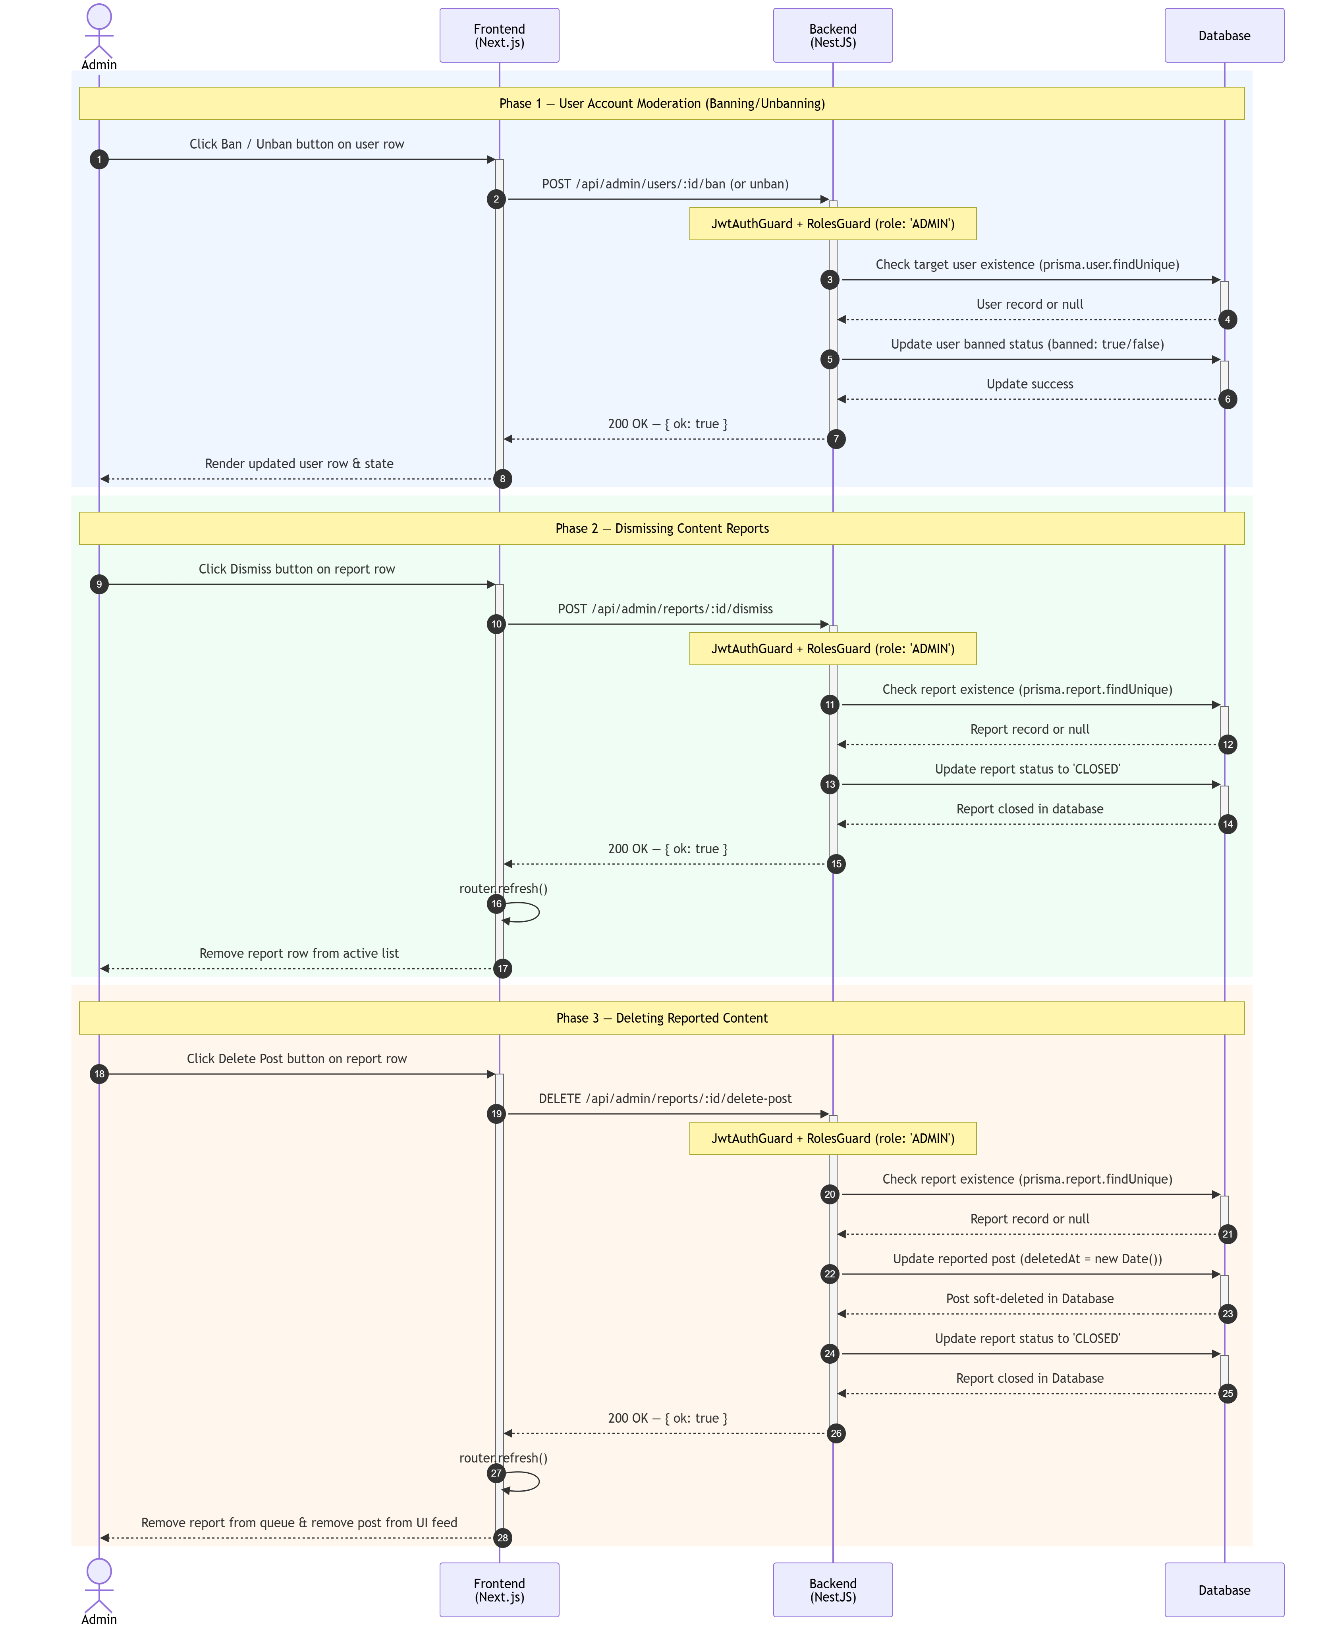
\includegraphics[width=0.92\linewidth,height=0.82\textheight,keepaspectratio]{images/image34.png}
  \caption{Administrative Moderation Diagram}
  \label{fig:29}
\end{figure}

\section{User Requirement Analysis:}

\subsection{User Interface Design:}

Breadit's user interface is split into two primary areas: a public-facing social network and a restricted administrative console. The user interface adapts a standardized three-column grid layout (navigation sidebar, central feed, and contextual discovery widgets) inspired by popular micro-blogging platforms like X/Twitter. This layout maximizes usability and reduces the learning curve for core social interactions. In contrast, the administrative panel uses a dark-themed dashboard focused purely on data visibility and moderation efficiency.

The client-side interface covers the user journey through the following main views:
\begin{itemize}
  \item Authentication \& Verification: Registration (Sign Up), login (Sign In), password recovery, and a 6-digit OTP verification view to validate email ownership.
  \item Unified Feed \& Discovery: Home timeline featuring "For You" (chronological) and "Explore" (trending by likes) tabs, supported by infinite-scroll hashtag feeds and a debounced search dropdown.
  \item Post Details \& Profiles: Individual post views with nested comment threads and media overlays, and user profiles containing filter tabs (Posts, Replies, Media{\ldots}).
  \item Messaging \& Communities: A real-time 1:1 chat interface powered by Socket.IO, and community pages featuring dedicated sub-feeds, group rules, and post submission queues.
  \item 
\end{itemize}

The moderation console contains two core operational views:
\begin{itemize}
  \item User Management (/admin-console/users): A searchable registry of users with controls to ban or reinstate suspended accounts.
  \item Content Moderation (/admin-console/reports): A real-time queue of flagged posts and comments, allowing admins to dismiss reports or delete offending content.
\end{itemize}

To maintain structural clarity and avoid redundant layouts in Chapter 3, mockups and user interface screenshots are excluded from this section and reserved for Chapter 5 (Demonstration). This section concentrates purely on design patterns and architectural user flows. Design inspirations and reference frameworks utilized in formulating the dashboard grid structure are acknowledged in the project bibliography, while screenshots of the deployed application in Chapter 5 document the actual system behavior.

\section{Technology Summary:}

This section provides a detailed overview of the technologies selected for the implementation of the full-stack micro-blogging and real-time social networking platform. While Chapter 2 outlined the theoretical concepts and general characteristics of modern web architectures, this section expands on those fundamentals by specifying their practical applications, architectural roles, and operational integration within the system. The integration of frontend, backend, caching, and database layers forms a cohesive, high-performance stack designed to support fast page rendering, real-time bidirectional communication, and provide an architectural foundation for the future integration of advanced trending and content trending/recommendation algorithms.

\subsection{Front -- end:}

\subsubsection{Technology Used: Next.js}

Next.js 15, powered by React 19, serves as the primary frontend framework for the platform. Utilizing the App Router architecture, Next.js combines Server-Side Rendering (SSR) for static content optimization with client-side interactivity, delivering a highly responsive, performant, and SEO-friendly social media interface.

\subsubsection{Architectural Role}

Next.js is responsible for:
\begin{itemize}
  \item Rendering page layouts and feeds (Home, Explore, Hashtags) dynamically.
  \item Managing user interaction states, including composing posts, liking content, commenting in threads, and updating profile settings.
  \item Communicating the NestJS backend via REST APIs for core CRUD transaction.
  \item Establishing a persistent Socket.IO connection to receive real-time notifications and handle instant messaging.
\end{itemize}

\subsubsection{Key Mechanisms and Features Applied}

\medskip\noindent\textbf{Server \& Client Component Architecture}\\[2pt]

The application leverages the separation of Server and Client components in. Static structures are pre-rendered on the server to optimize loading speeds, while interactive elements are modularized into client-side reusable components, such as:
\begin{itemize}
  \item Layout navigation: Leftbar (menu, user profile link) and Rightbar (search, trending, follow suggestion).
  \item Social interaction: Post (post/reposts), Comment (nested replies) and chat popups.
\end{itemize}

\medskip\noindent\textbf{State Management and Caching (TanStack Query)}\\[2pt]

To manage server state efficiently without complex global store boilerplate:
\begin{itemize}
  \item Instantly reflects actions (toggling a posts like status or following a user) in the UI before the backend confirmation completes, ensuring a zero-latency user experience.
  \item Caches user timelines, notification histories, and search results to prevent redundant API calls.
\end{itemize}

\medskip\noindent\textbf{Real-Time WebSocket Connection (Socket.IO)}\\[2pt]

For real-time features, the client maintains a persistent WebSocket connection.
\begin{itemize}
  \item Pushes real-time alerts (likes, follows, mentions, reposts) to users.
  \item Supports live, bidirectional transmission in the 1:1 chat interface, bypassing the overhead of traditional HTTP polling.
\end{itemize}

\medskip\noindent\textbf{Infinite Scrolling \& Asynchronous Fetching}\\[2pt]

To display long timelines without degrading browser performance, the application implements cursor-based pagination and infinite scrolling. As the next-page items are requested asynchronously, while skeleton screens are shown during data loading states.

\subsubsection{Justification}
\begin{itemize}
  \item Optimized Performance: Built-in features like route pre-fetching and asset optimization drastically reduce initial page load times.
  \item Architectural Flexibility: The modular, hook-driven architecture allows for easy expansion, making the codebase ready to integrate advanced content recommendation systems and trending pipelines in future phase.
\end{itemize}

\subsection{Back -- end:}

\subsubsection{Technology Used: NestJS (TypeScript) + Fastify}

NestJS, running on TypeScript and configured with Fastify as the underlying HTTP server adapter, serves as the main backend framework for the system. This combination provides a modular, highly scalable, and enterprise-grade architecture capable of handling intensive social media and real-time I/O workloads with high concurrency and low latency.

\subsubsection{Architectural Role}

The backend acts as the system's central business logic and data distribution layer:
\begin{itemize}
  \item Handles user session state and authentication (JWT cookie-based authentication)
  \item Manages core social networking domain workflows (feed query generation{\ldots})
  \item Manages database transaction and query logic PostgreSQL via Prisma ORM client.
  \item Dispatches real-time events (likes,notifications,messages) using Socket.IO gateways.
  \item Restricts API access via Guards, Pipes, and Throttling middleware.
\end{itemize}

\subsubsection{Key Mechanisms and Features Applied}

\medskip\noindent\textbf{High-Performance Asynchronous I/O (NestJS + Fastify)}\\[2pt]

Instead of standard Express engines, NestJS is configured with Fastify to support rapid asynchronous I/O execution. This enables:
\begin{itemize}
  \item Fast handling of simultaneous HTTP requests under high traffic.
  \item Efficient processing of pagination queries for massive feeds.
  \item Low-overhead file streaming and media uploads (Fastify's multipart performance).
\end{itemize}

\medskip\noindent\textbf{DTO-Based Data Validation (Class Validator \& Pipes)}\\[2pt]

All incoming API requests go through NestJS ValidationPipes:
\begin{itemize}
  \item Utilizes class-validator and class-transformer to enforce strict DTO (data transfer object) schemas.
  \item Sanitizes input and rejects malformed payloads before they reach service methods, preventing injection attacks and ensuring data integrity.
\end{itemize}

\medskip\noindent\textbf{Modular Architecture \& REST Services}\\[2pt]

The backend is divided into specialized modules (Auth, Users, Posts, Messages, Notifications, Communities) adhering to NestJS's dependency injection principles:
\begin{itemize}
  \item Exposes structured RESTful endpoints (POST /api/auth/register, GET /api/posts/feed
  \item Separates database operations using Prisma client services.
  \item This design supports future migration into isolated microservices if necessary.
\end{itemize}

\medskip\noindent\textbf{Integration with the Trendng/Recommendation Engine}\\[2pt]

\medskip\noindent\textbf{Real-time Event Broadcasting (Socket.IO + Redis Adapter)}\\[2pt]

To support instant notifications and direct messages, the backend implements:
\begin{itemize}
  \item WebSocket Gateways: Encapsulated within Socket.IO gateways to manage client WebSocket sessions.
  \item Redis Adapter: Utilizes redis-adapter to synchronize WebSocket events across multiple server instances, ensuring horizontal scaling.
\end{itemize}

\subsubsection{Justification}

NestJS + Fastify was chosen due to:
\begin{itemize}
  \item Modular and Scalable Structure: Dependency injection and module design result in a highly testable and maintainable codebase.
  \item Substantial Performance Gains: Fastify handles up to two times more requests per second compared to Express, offering optimal resource utilization.
  \item Robust Database Integration: Prisma ORM provides type-safe query building, auto-generated migrations, and high developer velocity.
  \item Ready for Future Scale: The architectural decoupling of services and the integration of Redis adapters ensure the system can scale both vertically and horizontally, easily accommodating real-time recommendation engines or dedicated feed-processing workers in future iterations.
\end{itemize}

\subsection{Database:}

The system incorporates a hybrid storage architecture combining a relational database with an in-memory data store to optimize transactional consistency, real-time state synchronization, and low-latency cache queries.

\subsubsection{Relational Database: PostgreSQL}

\medskip\noindent\textbf{Architectural Role}\\[2pt]

PostgreSQL-the primary relational database, stores all structured application entities:
\begin{itemize}
  \item User Identity \& Relations: Accounts, profile data, bidirectional follow/block relationships.
  \item Content \& Interactions: Posts, media attachments, nested comments, likes, saves, and report logs.
  \item Messaging \& Communities: 1:1 direct messages, conversation memberships, and community settings (rules, bans).
\end{itemize}

\medskip\noindent\textbf{Why PostgreSQL}\\[2pt]
\begin{itemize}
  \item Strong ACID Compliance: Guarantees transaction reliability for user registrations, authentication flows, and content states.
  \item Advanced Relational Modeling: Supports complex self-referencing structures essential for nested comments and reposts.
  \item Seamless ORM Compatibility: Integrates cleanly with Prisma ORM for automated schema migrations and type-safe database queries.
\end{itemize}

\medskip\noindent\textbf{Applied Features}\\[2pt]
\begin{itemize}
  \item Data Integrity Constraints: Unique constraints on fields and compound keys for relationship records.
  \item Query Optimization: Custom indexes on frequently queried fields to speed up timeline rendering.
  \item Atomic Transactions: Atomic database writes via Prisma Transaction APIs to register multiple related records simultaneously.
\end{itemize}

\subsection{Deployment}

The Breadit system is designed to be deployed in a cloud environment using the PaaS (Platform as a Service) and Serverless models. Specialized cloud services help minimize infrastructure management overhead, automate the CI/CD (Continuous Integration/Continuous Deployment) pipeline, and optimize performance for each application component.

The physical deployment architecture consists of the following components:
\begin{itemize}
  \item Frontend (Next.js): Deployed on Vercel (Serverless \& CDN).
  \item Backend (NestJS): Deployed on Render (Containerized Web Service).
  \item Database (PostgreSQL): Manage database service provided by Supabase.
  \item Cache (Redis): The Serverless Redis service provided by Upstash.
  \item Media Storage \& CDN: The cloud storage and media delivery services of Cloudinary.
\end{itemize}

\subsubsection{Workflow}
\begin{center}
  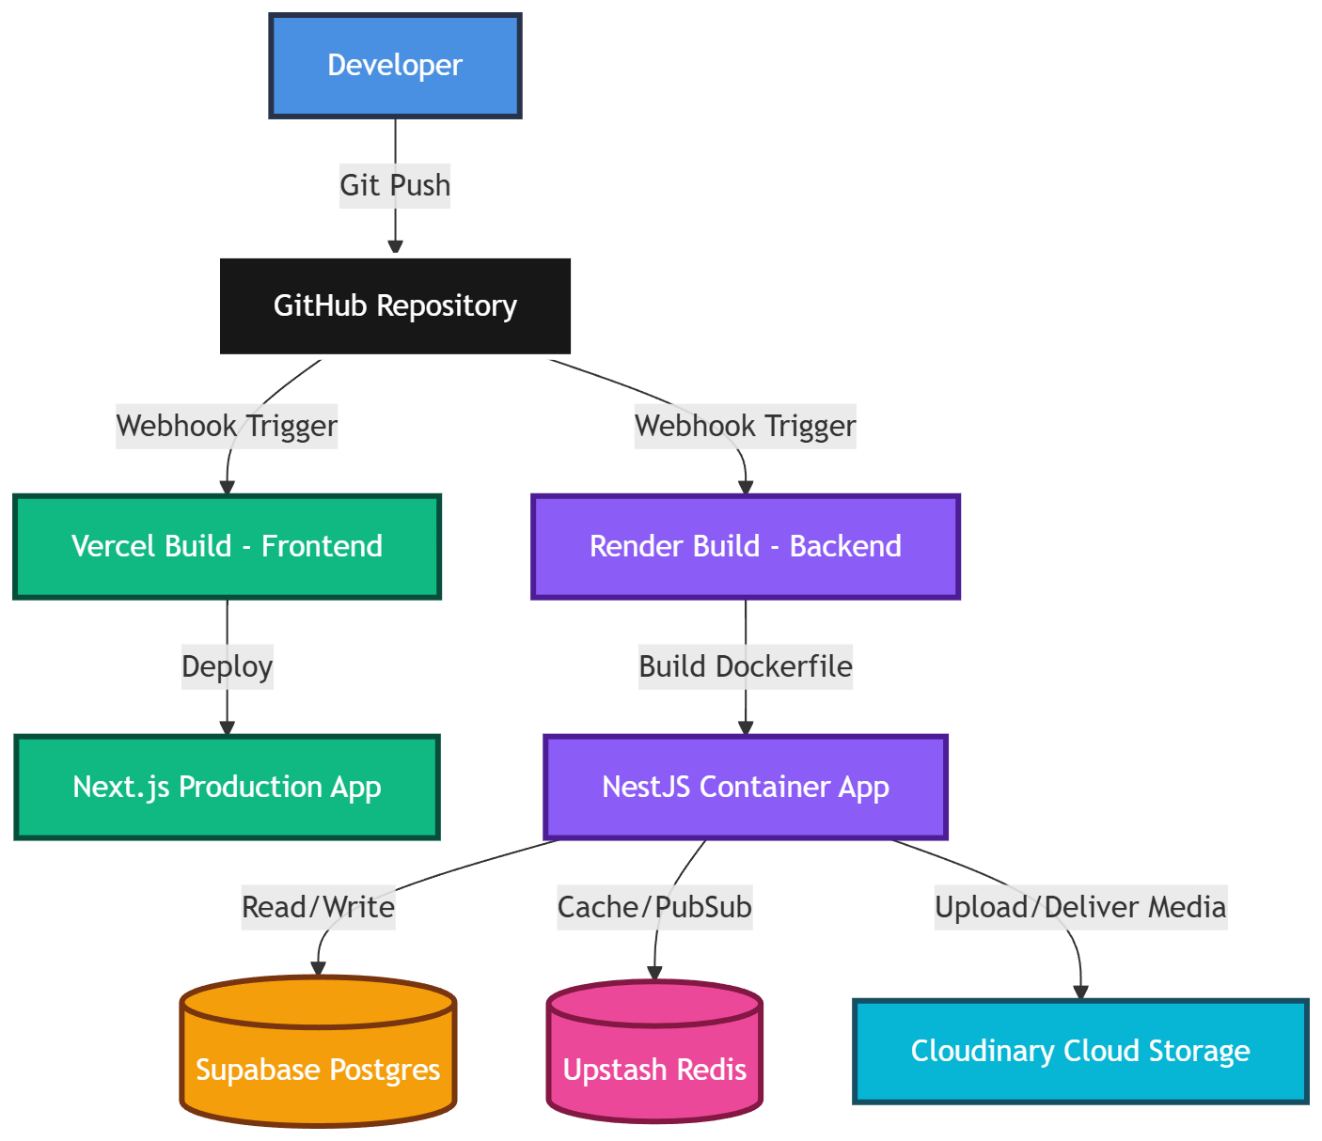
\includegraphics[width=0.92\linewidth,height=0.82\textheight,keepaspectratio]{images/image35.png}
\end{center}

\medskip\noindent\textbf{Flow A: (Frontend)}\\[2pt]
\begin{itemize}
  \item Trigger: The developer pushes new source code to the main branch of the GitHub repository.
  \item Build Pipeline: Vercel detects modifications within the frontend directory (apps/frontend/). An automated build pipeline is triggered on Vercel's infrastructure:
\begin{itemize}
  \item Node.js environment initialization.
  \item Compiling Next.js source code to a production-ready build (optimizing static pages, server-side routes, and minifying assets).
\end{itemize}
  \item Deployment: Once compilation succeeds, the build artifact is deployed and distributed across Vercel's global Edge CDN network. Vercel's router seamlessly redirects user traffic to the new version without any downtime.
\end{itemize}

\medskip\noindent\textbf{Flow B: (Backend)}\\[2pt]
\begin{itemize}
  \item Trigger: Similarly, a push event to the main branch fires a webhook targeting Render.
  \item Docker Build: Render identifies changes in the backend directory (apps/backend/) and reads the configured Dockerfile (apps/backend/Dockerfile):
\begin{itemize}
  \item A multi-stage Docker build runs to minimize the final container image size.
  \item Environment variables such as DATABASE\_URL (pointing to Supabase) and REDIS\_URL (pointing to Upstash) are injected during runtime.
\end{itemize}
  \item Deploy Container: Render spawns the NestJS backend container from the compiled Docker image. It performs continuous health checking via the /api/health endpoint. Once the container responds with a healthy status (200 OK), Render routes incoming API traffic to the new container and safely terminates the deprecated instance.
\end{itemize}

\subsubsection{Networking and Security}
\begin{itemize}
  \item Transport Layer Security (HTTPS/WSS): All connections from user browsers to the Frontend (Vercel) and Backend (Render) are strictly encrypted using HTTPS and WSS (Secure WebSockets). SSL/TLS certificates are provisioned and auto-renewed Encrypt.
  \item CORS (Cross-Origin Resource Sharing): The NestJS backend enforces a strict CORS policy, authorizing only requests originating from the official Frontend domain access API resources.
  \item Database Isolation: PostgreSQL on Supabase and Redis on Upstash are secured behind complex password authentication mechanisms and require SSL-encrypted connections. Database access ports are tightly restricted and shielded from the public internet.
  \item Authentication Security: JWT authentication tokens are securely transmitted between client and server via Cookies configured with the httpOnly flag (mitigating XSS token theft risks) and the Secure flag (restricting transmissions to HTTPS connections only).
\end{itemize}

\subsubsection{Compute and Scalability}
\begin{itemize}
  \item Frontend Compute: Leveraging Vercel's serverless infrastructure, static assets are cached at Edge nodes. Serverless API functions scale up and down instantly to accommodate fluctuating user traffic without manual configuration.
  \item Backend Compute: The NestJS container instance running on Render is continuously monitored for CPU and memory utilization. Under high load, Render supports both vertical scaling (allocating more CPU/RAM resources) and horizontal scaling (replicating multiple container instances running in parallel).
  \item Caching \& Load Reduction: The integration of Upstash Redis allows heavy queries (such as the Trending Feed) to be cached. This significantly alleviates processing overhead on the NestJS backend CPU and reduces direct read IOPS on the primary PostgreSQL database.
\end{itemize}

\subsubsection{Database Service}
\begin{itemize}
  \item The primary data layer of Breadit is powered by Supabase (Managed PostgreSQL):
\begin{itemize}
  \item Database Engine: PostgreSQL 16 running on optimized cloud infrastructure.
  \item Role: Stores structured data across the system, including User Profiles, Posts, Comments, Communities (Sub-breadits), Votes, and Moderation Reports.
  \item Automated Management: Features automated daily backups and Connection Pooling (via PgBouncer/Supabase Pooler) to sustain thousands of concurrent connections from the Backend without exhausting system resources.
  \item ORM Integration: Integrates seamlessly with Prisma ORM on the backend to synchronize schema definitions and execute database migrations safely.
\end{itemize}
\end{itemize}
